\documentclass[10pt,aspectratio=149]{beamer}
\usecolortheme{Calm}
\usetheme{Calm}
%\usefonttheme[onlymath]{serif} % beamer force les maths en cmss par défaut, qui n'a pas de vrai gras : \mathbf{} restait fin
\usepackage{amsmath}
\usepackage{pgfplots}
\pgfplotsset{compat=1.18}
\usepackage{pgfplotstable}
\usepackage[utf8]{inputenc}
\usepackage{hyperref}
\RequirePackage[absolute,overlay]{textpos}
%\usepackage[sfdefault]{cabin}
%\usepackage[T1]{fontenc}
%\setlength{\TPHo{}rizModule}{\paperwidth}
%\setlength{\TPVertModule}{\paperheight}
%\definecolor{OQEdarkblue}{HTML}{046085}


\defbeamertemplate*{background canvas}{bg}
{%
  \color{lightgray!40}\vrule width\paperwidth height\paperheight% added bg color
}

% Centered, larger display equation
\newcommand{\keyeq}[1]{%
  \begin{center}
    \Large$\displaystyle #1$
  \end{center}%
}

% Same style, for a system of equations aligned on "="
% (rows separated by \\, each row written as LHS &= RHS)
\newcommand{\keyeqs}[1]{%
  \begin{center}
    \normalsize$\displaystyle
    \begin{aligned}
    #1
    \end{aligned}
    $
  \end{center}%
}

%------------------------------

\author{Dominique Gravel}
\title{Trophic metacommunities}
\date{August 27th, 2026}
\institute{Université de Sherbrooke \\ Summer school in biodiversity modelling}

%------------------------------
% TITLE SLIDE
%------------------------------

\usebackgroundtemplate
{
  
\includegraphics[width=\paperwidth,height=\paperheight]{bg}%
}

\begin{document}

	\begin{frame}[plain]
		\titlepage
	\end{frame}

%------------------------------
% INTRO
%------------------------------

\begin{frame}

    \begin{center}
        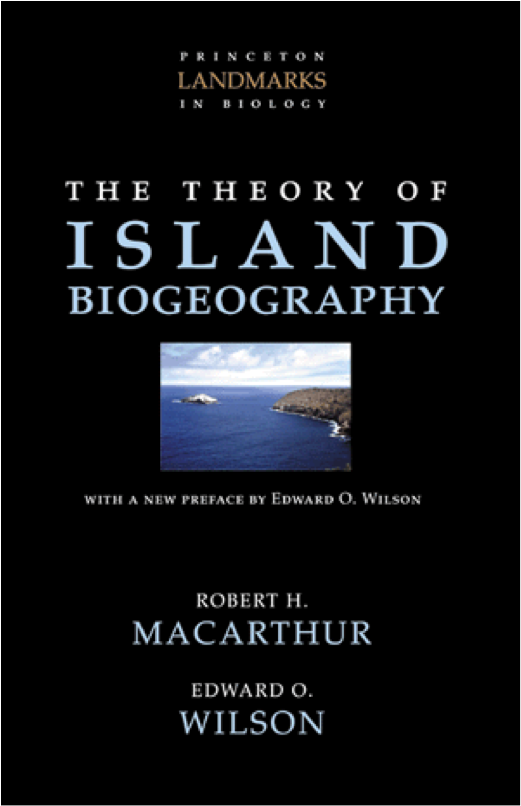
\includegraphics[height=0.8\textheight]{Figs/IBT_cover}\\
    \end{center}

\end{frame}

%------------------------------

\begin{frame}

	\begin{columns}
		\begin{column}{0.5\textwidth}
            \begin{center}
                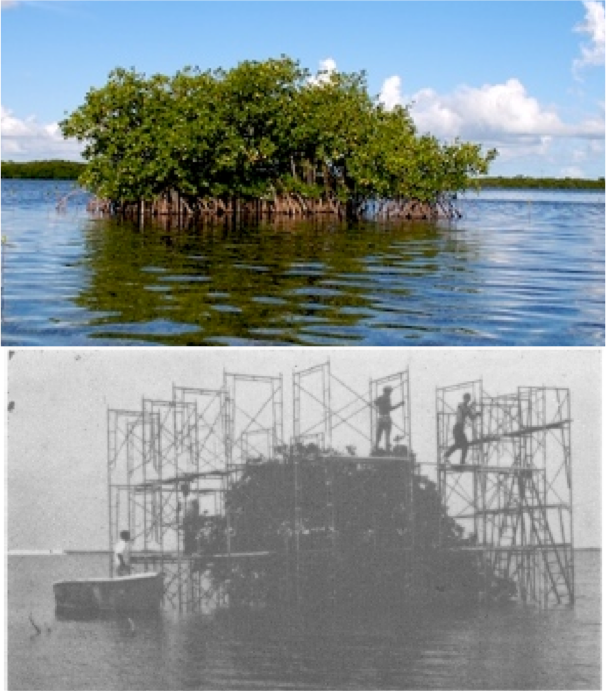
\includegraphics[height=0.7\textheight]{Figs/experiment} 
            \end{center}
		\end{column}
%----
		\begin{column}{0.5\textwidth}
            \begin{center}
                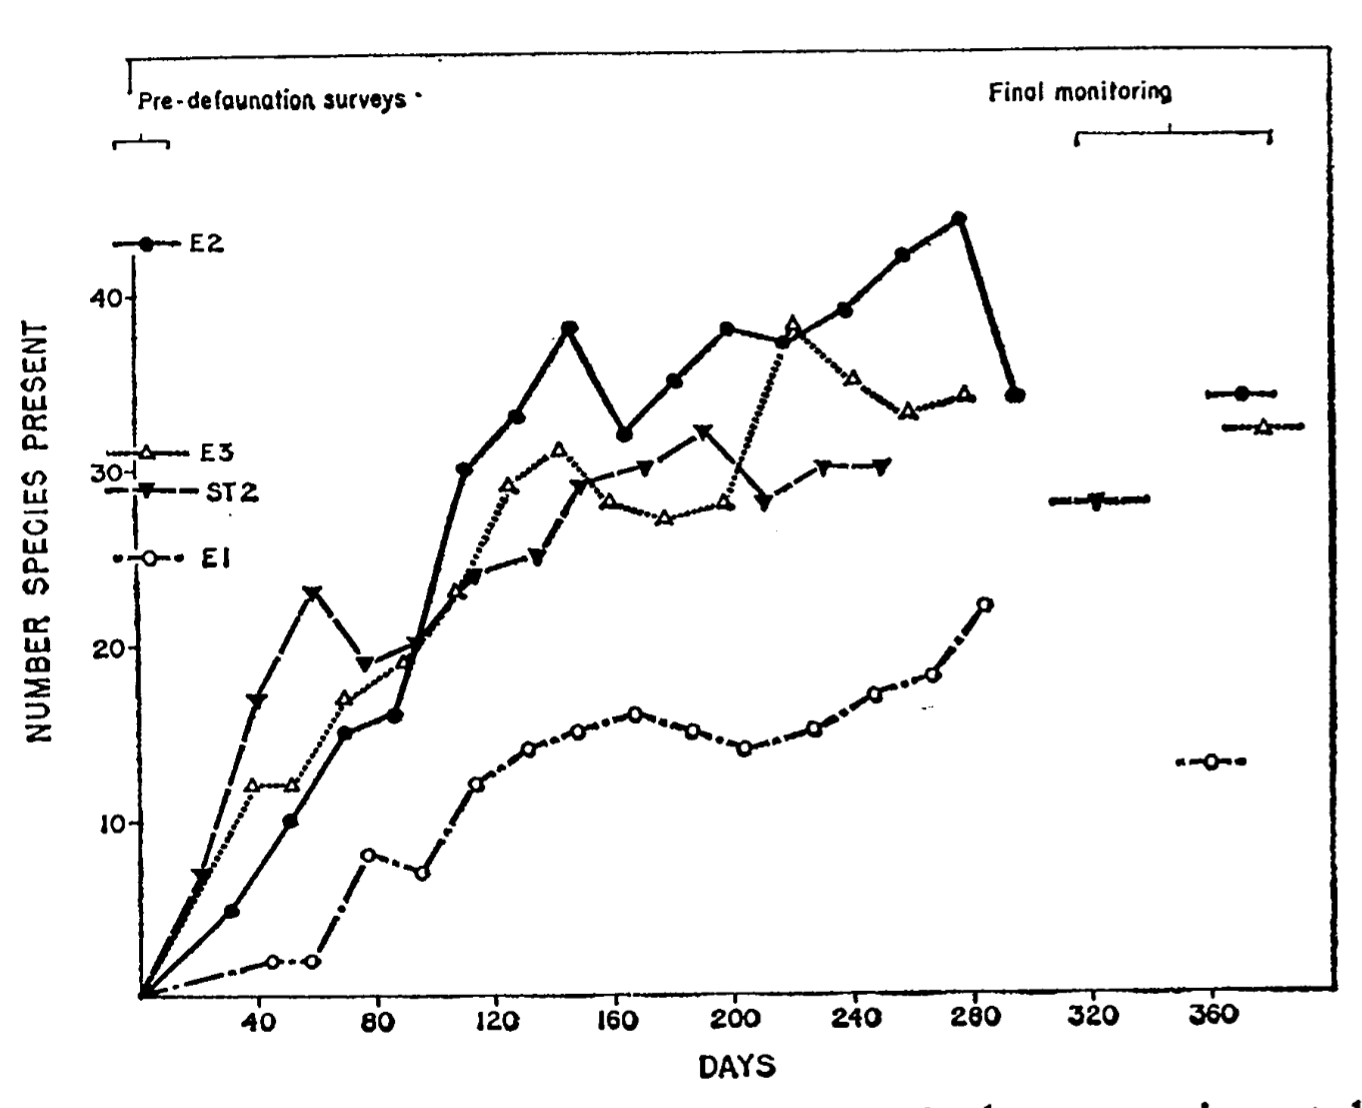
\includegraphics[height=0.6\textheight]{Figs/simberloff1967}\\
                \footnotesize Simberloff and Wilson, 1967, 1969. Ecology. 
            \end{center}
		\end{column}
	\end{columns}

\end{frame}

%------------------------------

\begin{frame}{Classic IBT}{Graphical theory}

    \begin{center}
        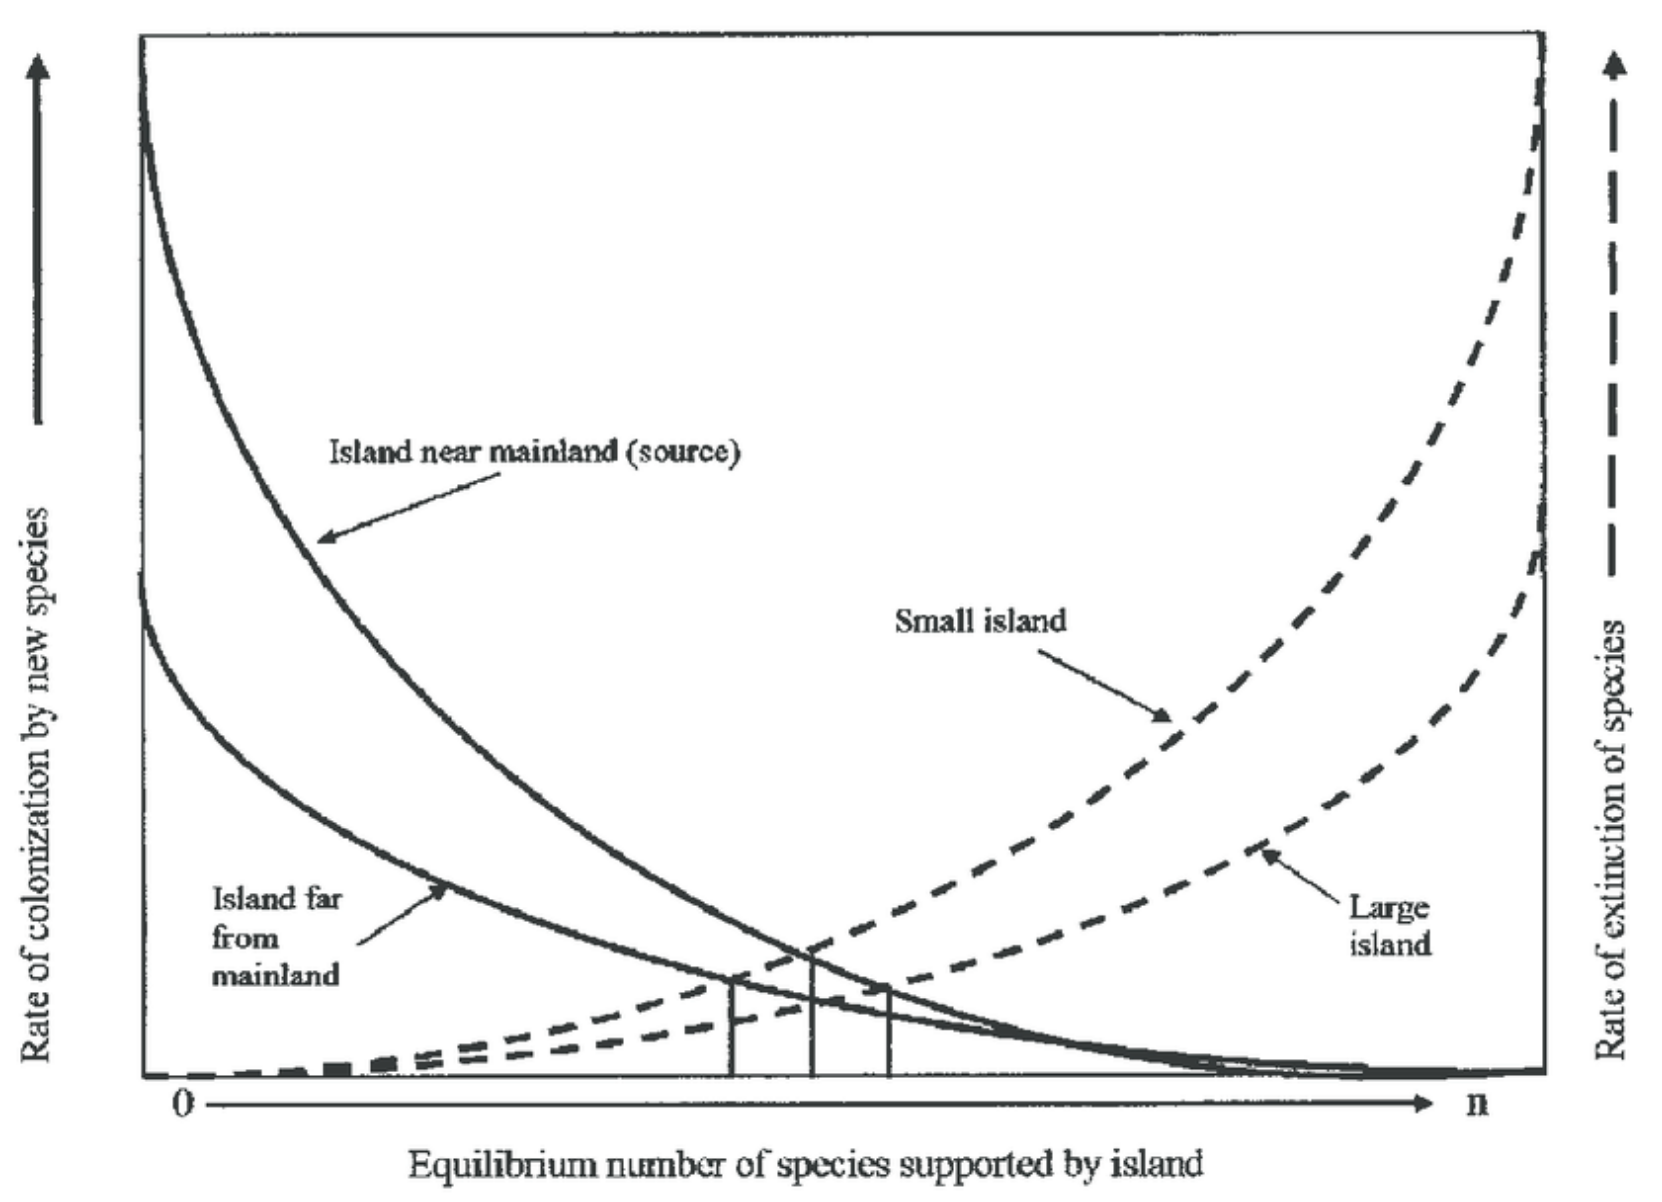
\includegraphics[height=0.7\textheight]{Figs/IBT}\\
    \end{center}

\end{frame}

%------------------------------

\begin{frame}{Classic IBT}{Model}

    Very similar to the Levins model : 
        \keyeqs{\frac{dp}{dt} = c(1-p) - ep}

    With solution
        \keyeqs{p^* = \frac{c_i}{c+e}}

    And
        \keyeqs{S^* = P p^* = P\frac{c_i}{c+e}}

\end{frame}

%------------------------------

\begin{frame}{Classic IBT}{Lessons}

    \begin{itemize}
        \item Importance of colonization and extinction dynamics
        \item Local communities are sampled from the regional pool
        \item Dynamic equilibrium
        \item Hypothesis for species-area relationship
        \item Speculations on evolutionary dynamics
    \end{itemize}

\end{frame}

%------------------------------


\begin{frame}{Classic IBT}{Limits}

    A community is more than a species list

    \begin{center}
        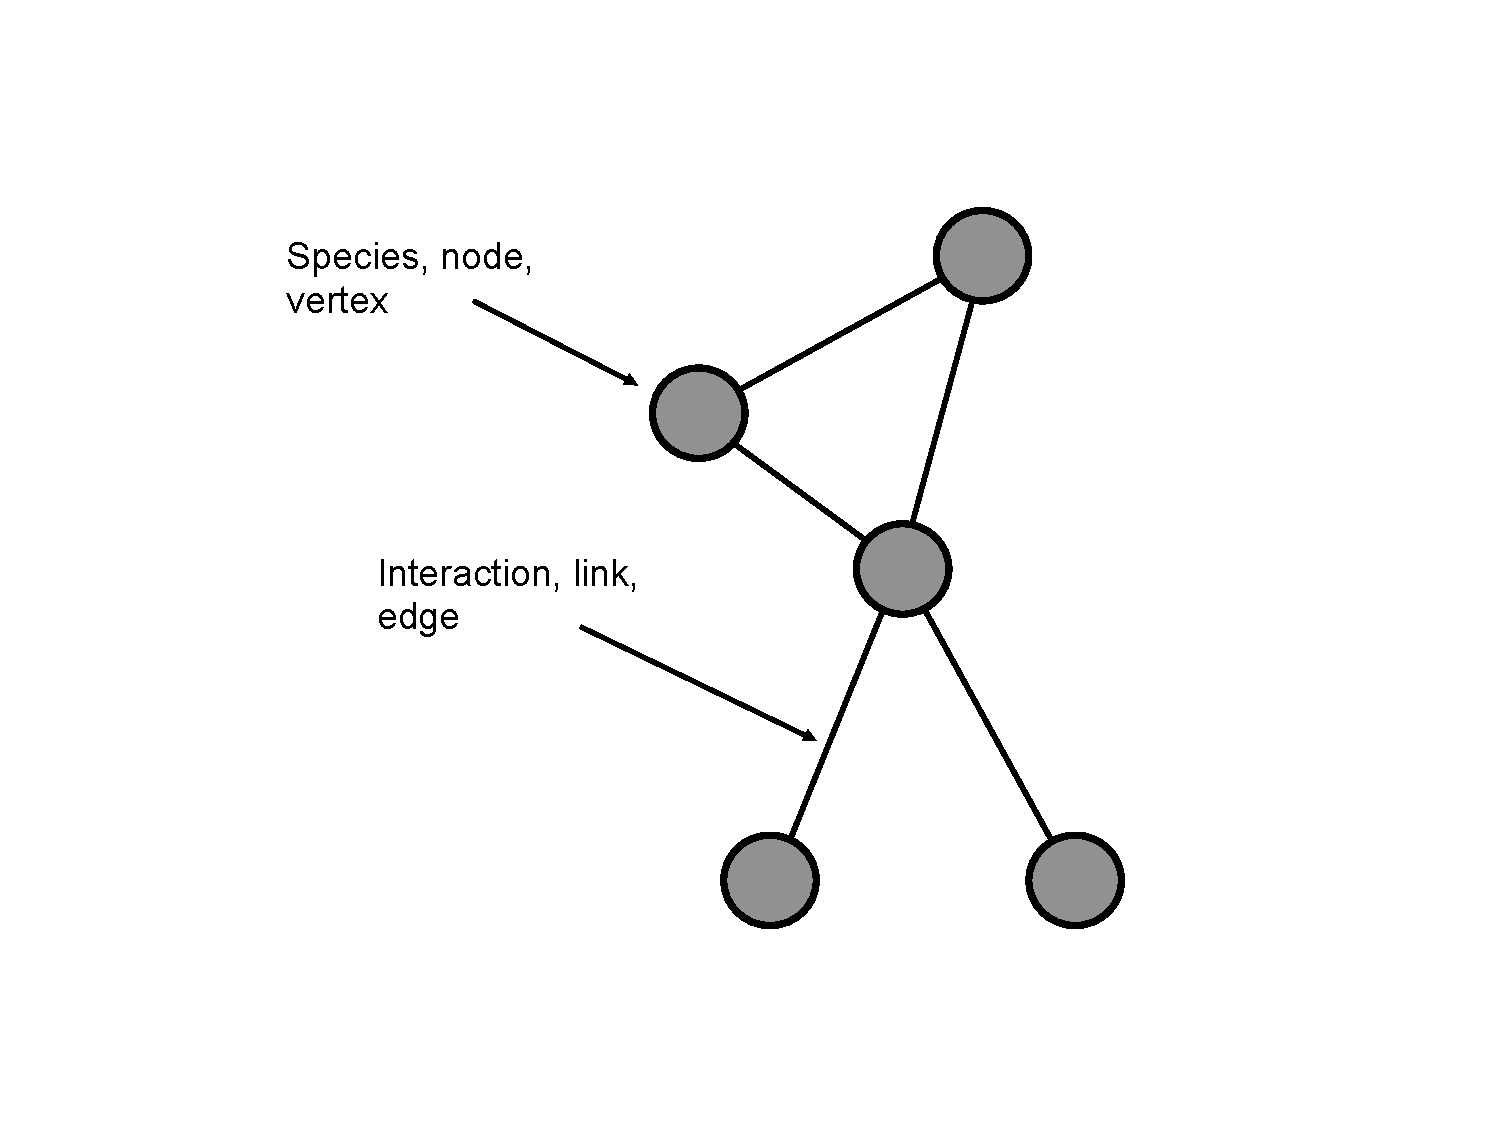
\includegraphics[height=0.7\textheight]{Figs/network}\\
    \end{center}

\end{frame}

%------------------------------

\begin{frame}{Classic IBT}{Limits}

    \begin{center}
        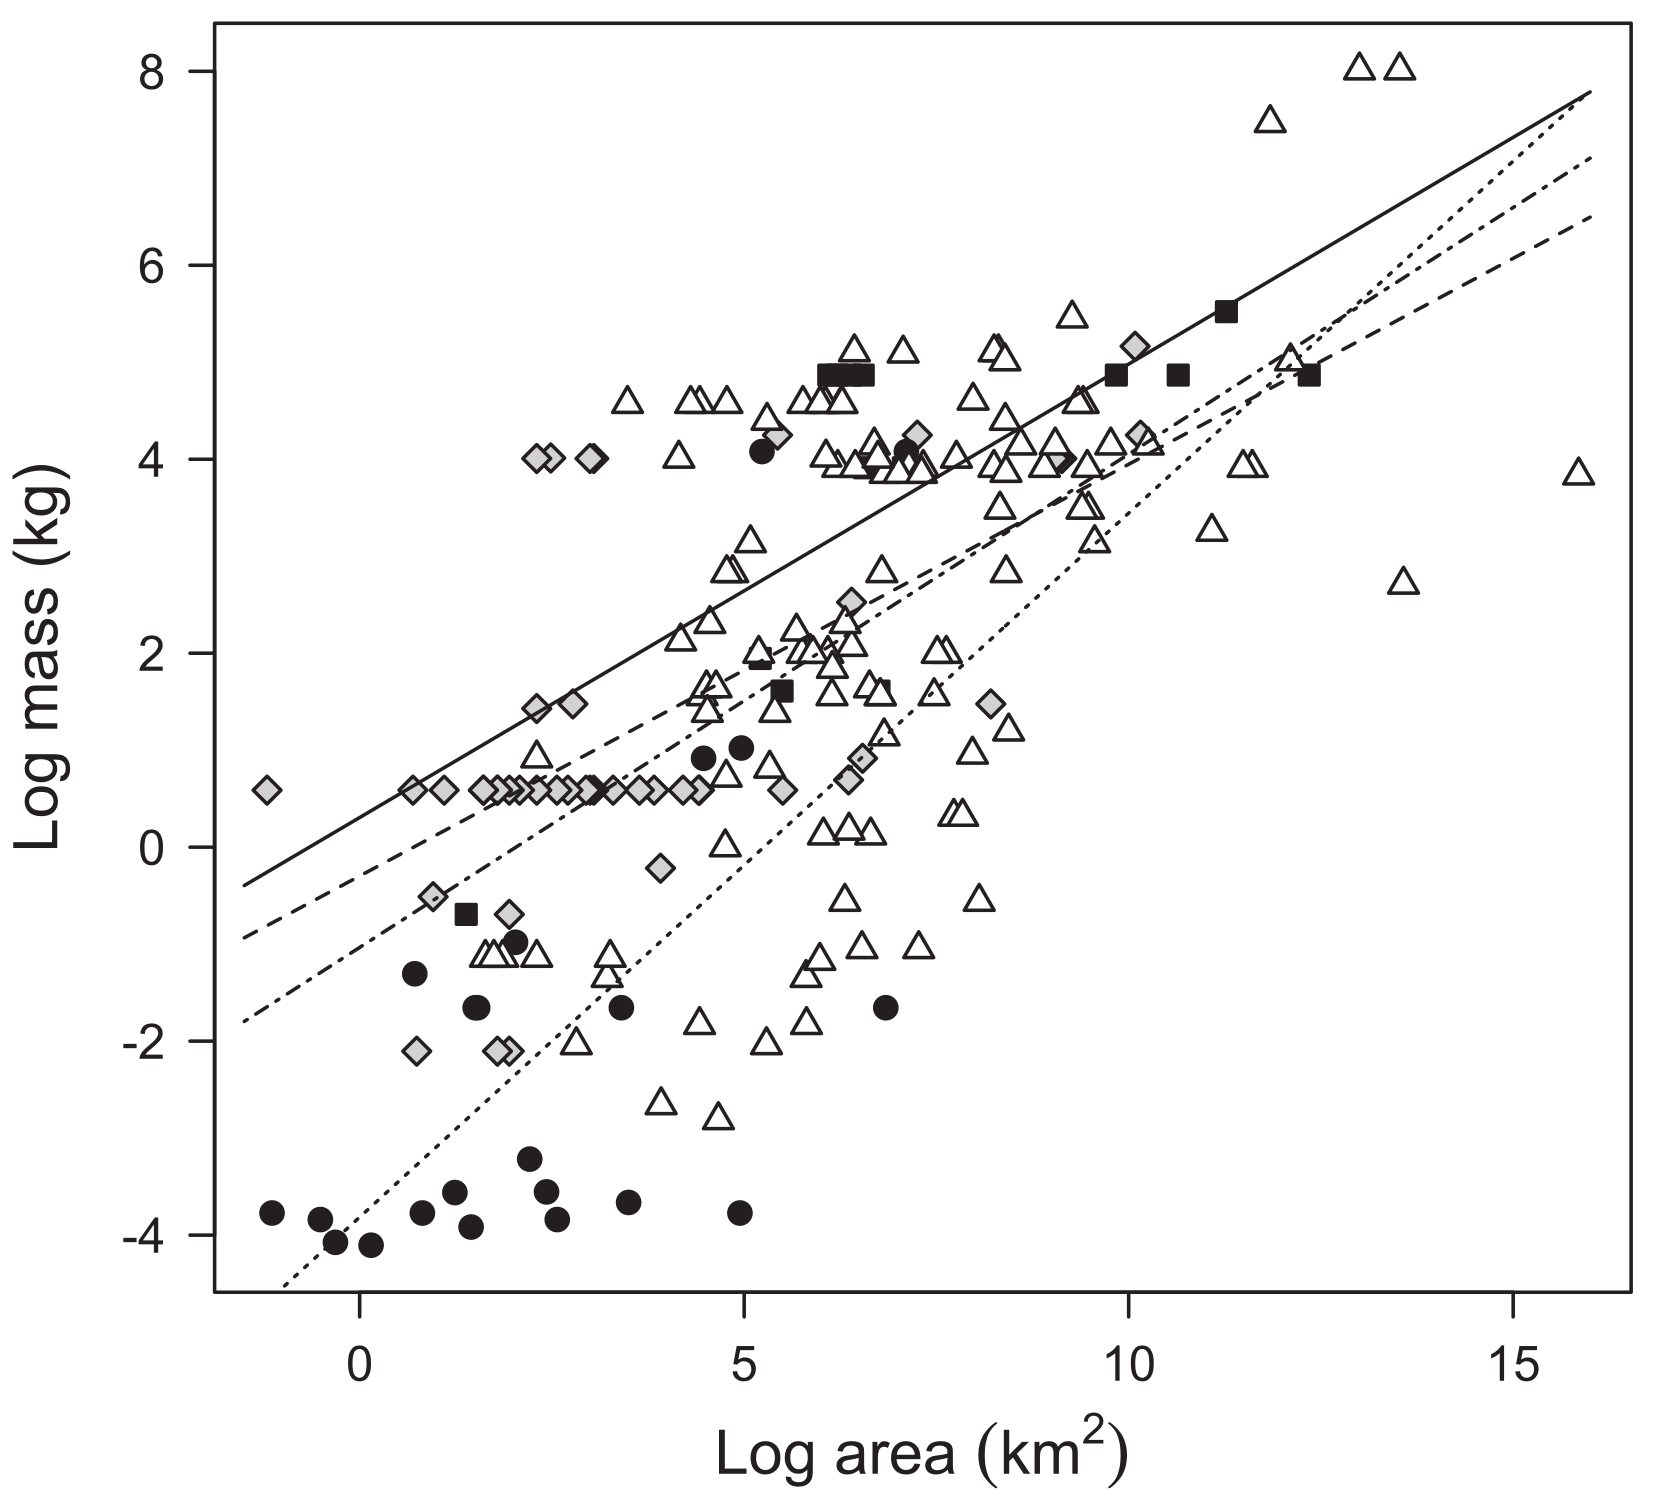
\includegraphics[height=0.7\textheight]{Figs/millien2011b}\\
        \footnotesize Millien and Gonzalez. 2011. JBiog.
    \end{center}

\end{frame}

%------------------------------
% IBT Exercise
%------------------------------

{
\usebackgroundtemplate{}
\begin{frame}

	\pagecolor{BDQC1st}
	\color{white}

	\LARGE{\textit{Exercise}}

\end{frame}
}

%------------------------------

\begin{frame}{Classic IBT}

    Simulate community assembly dynamics on islands without ecological interactions. 
    
    Explore the effect of island size and distance to mainland on 

    \begin{itemize}
        \item Time it takes to reach equilibrium
        \item Species turnover after equilibrium 
    \end{itemize}

\end{frame}

%------------------------------

\begin{frame}{Classic IBT}{Specialized interactions}

    \begin{itemize}
        \item Now consider a regional pool of plants ($P$) and of herbivores ($H$)
        \item Plants do not have any constraint to colonize islands       
        \item Herbivore species $j$ requires plant species $i=j$ to be present on the island to colonize
        \item Herbvirore species $j$ goes extinct if plant species $i=j$ goes extinct
    \end{itemize}

    What is the equilibrium species richness of plants and herbivores ?

\end{frame}

%------------------------------
% Predator-prey assembly
%------------------------------

{
\usebackgroundtemplate{}
\begin{frame}

	\pagecolor{BDQC1st}
	\color{white}

	\LARGE{\textit{Predator-prey assembly}}

\end{frame}
}

%------------------------------

\begin{frame}{Levins model}{Two trophic levels}

    Let's first consider a two trophic levels model where the predator requires the presence of the prey to occpuy a patch. We have the general equation for trophic level $l$:

    \keyeqs{\frac{dp_l}{dt} = c_lp_l(h_l-p_l) - e_lp_l}

    where $h_l$ is the fraction of patches suitable for that species, i.-e. the occupancy of the lower trophic level ($h_2 = p_1$).

    We call this model "donor-controlled" because it is the lower trophic level that determines the dynamics of higher level, without top-down regulation. 
\end{frame}

%------------------------------

\begin{frame}{Levins model}{Two trophic levels}

    From basic metapopulation theory we know that 

    \keyeqs{p_1^* = 1 -\frac{e_1}{c_1}}

    And solving for the higher trophic level we get 

    \keyeqs{p_2^* = h_2 -\frac{e_2}{c_2} = 1 -\frac{e_1}{c_1} -\frac{e_2}{c_2}}

    With this formulation, it is easy to gess that the second trophic level requires that $e_2/c_2 < 1 - e_1/c_1$ for persistence

\end{frame}

%------------------------------

\begin{frame}{Concept of spatial inefficiency}

    \begin{center}
        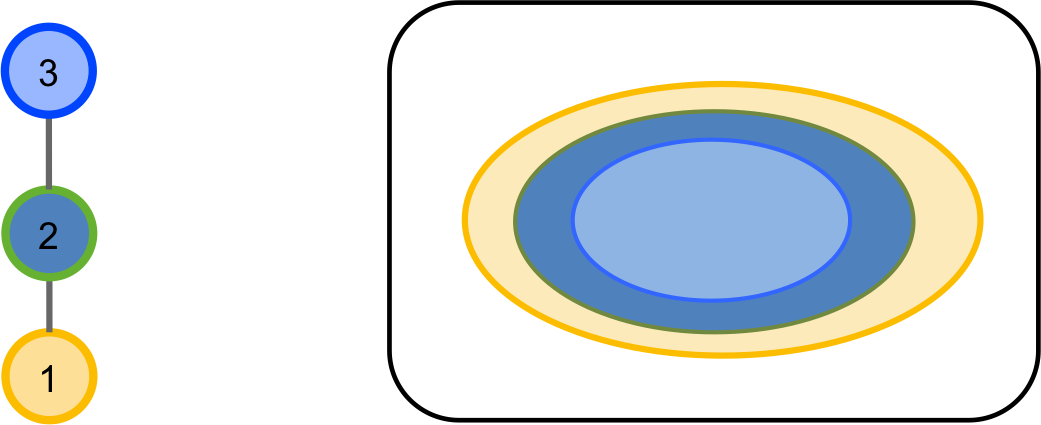
\includegraphics[height=0.5\textheight]{Figs/spatial_inefficiency}\\
    \end{center}

\end{frame}

%------------------------------

\begin{frame}{Limits to food chain length}

    Taking this reasonning to multiple trophic levels, we get the condition for persistence of trophic level $n$ :

    \keyeqs{h_1 > \sum_{j=1}^n \frac{e_j}{c_j}}

    From which we can derive three conclusions
    \begin{enumerate}
        \item All things equal, occupancy should decrease with trophic level
        \item Spatial dynamics imposes a limit to food chain length
        \item Selection should promote larger colonization and lower extinction with increasing trophic level
    \end{enumerate}

\end{frame}

%------------------------------

\begin{frame}{Concept of spatial inefficiency}{Spatial use properties}

	\begin{columns}
		\begin{column}{0.5\textwidth}

		\end{column}
%----
		\begin{column}{0.5\textwidth}
            \begin{center}
                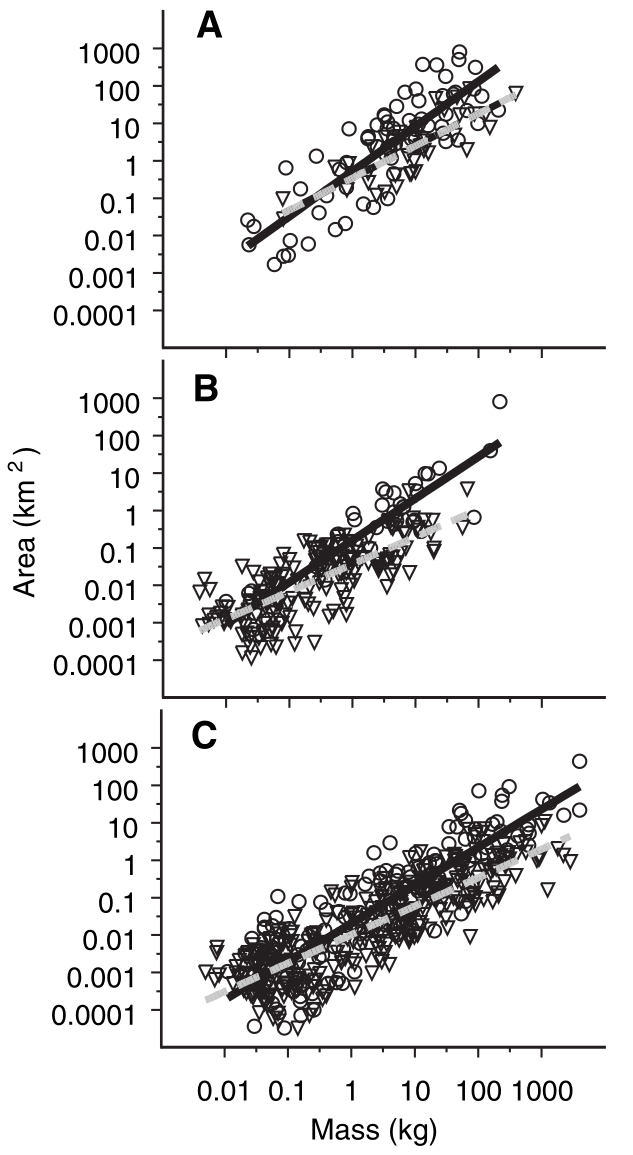
\includegraphics[height=0.7\textheight]{Figs/jetz2004}\\
                \footnotesize Jetz et al. 2004. Science  
            \end{center}
		\end{column}
	\end{columns}

\end{frame}

%------------------------------

\begin{frame}{Concept of spatial inefficiency}{Spatial use properties}

	\begin{columns}
		\begin{column}{0.5\textwidth}
            \begin{itemize}
                \item Dispersal distance
                \item Foraging (home range)
                \item Migration distsance
            \end{itemize}
		\end{column}
%----
		\begin{column}{0.5\textwidth}
            \begin{center}
                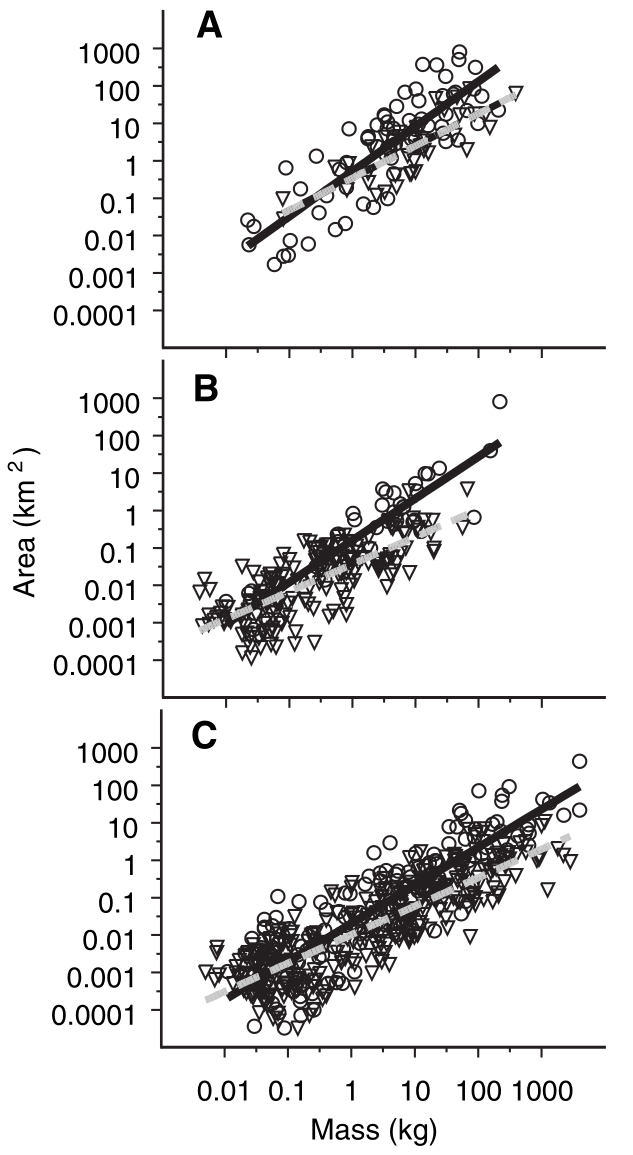
\includegraphics[height=0.7\textheight]{Figs/jetz2004}\\
                \footnotesize Jetz et al. 2004. Science 
            \end{center}
		\end{column}
	\end{columns}

\end{frame}

%------------------------------

\begin{frame}{Concept of spatial inefficiency}{Spatial use properties}

	\begin{columns}
		\begin{column}{0.5\textwidth}
            \begin{itemize}
                \item Dispersal distance
                \item Foraging (home range)
                \item Migration distsance
            \end{itemize}
		\end{column}
%----
		\begin{column}{0.5\textwidth}
            \begin{center}
                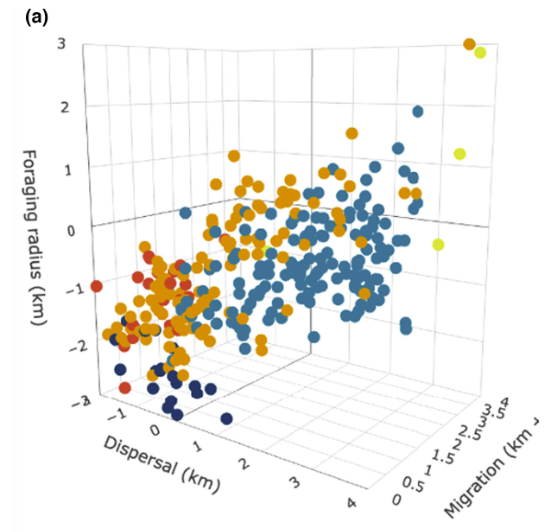
\includegraphics[height=0.7\textheight]{Figs/straus2024}\\
                \footnotesize Straus et al. 2024. GEB. 
            \end{center}
		\end{column}
	\end{columns}

\end{frame}

%------------------------------

\begin{frame}{Concept of spatial inefficiency}{Diet breadth}

    \begin{center}
        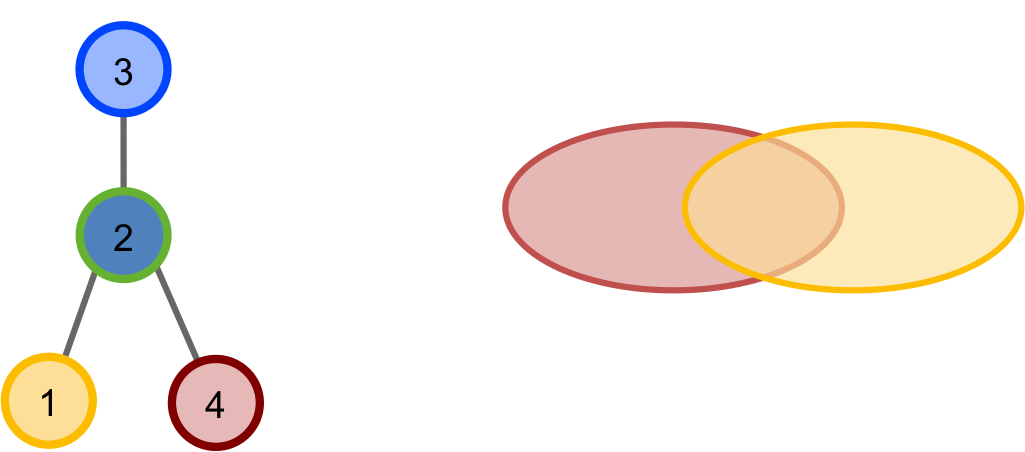
\includegraphics[height=0.5\textheight]{Figs/prey_diversity}\\
    \end{center}

\end{frame}

%------------------------------

\begin{frame}{Concept of spatial inefficiency}{Diet breadth}

    \begin{center}
        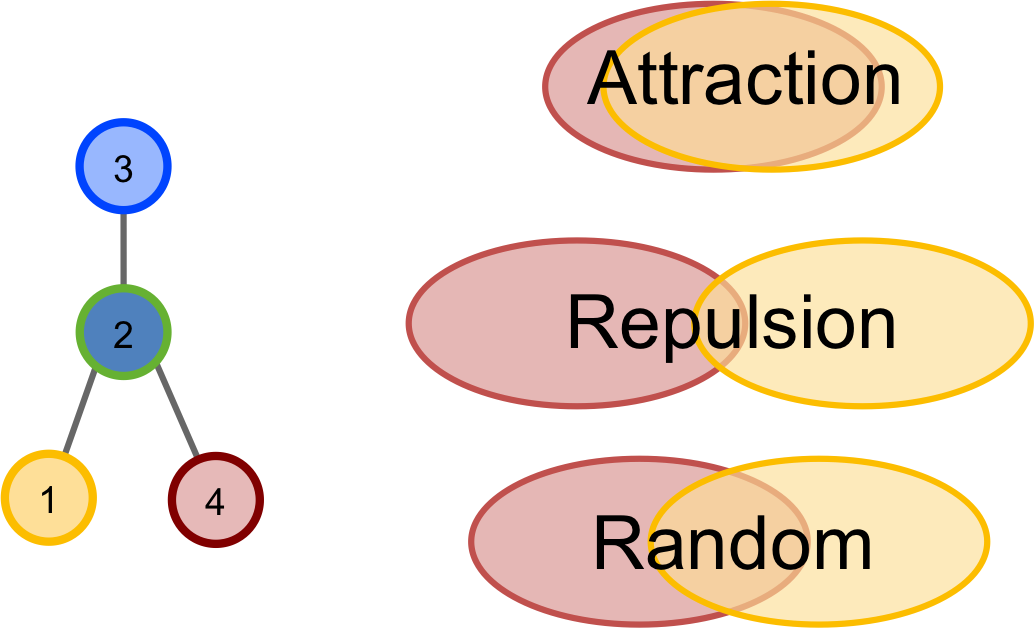
\includegraphics[height=0.5\textheight]{Figs/prey_codistribution}\\
    \end{center}

\end{frame}

%------------------------------

\begin{frame}{Concept of spatial inefficiency}{Summary}

    \begin{center}
        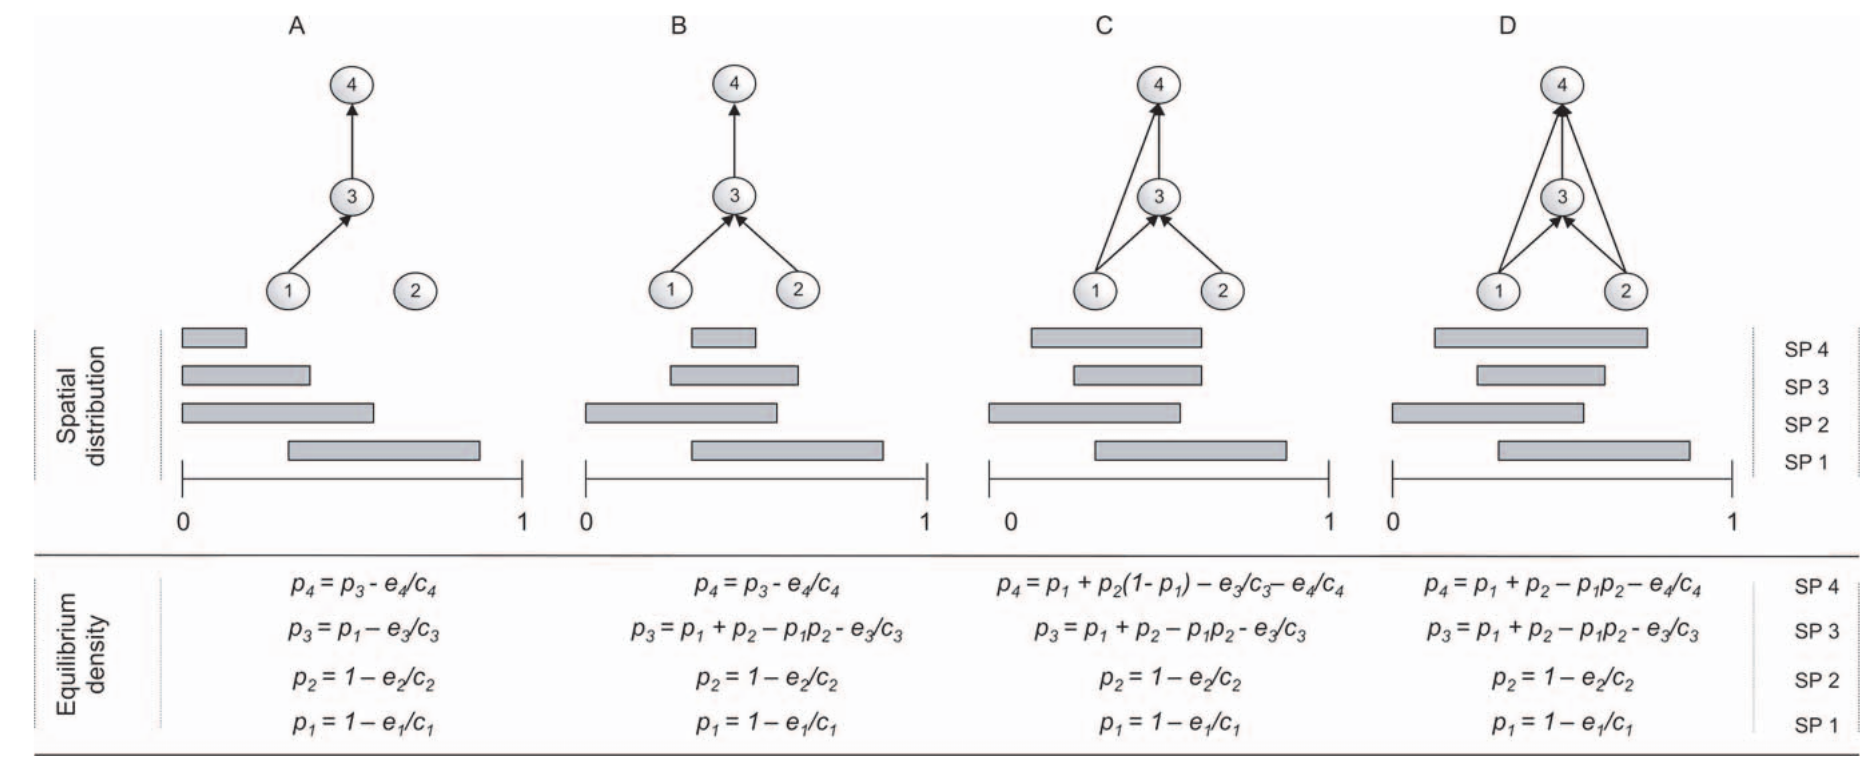
\includegraphics[height=0.55\textheight]{Figs/gravel2011a}\\
        \footnotesize Gravel et al. 2011. PLOS ONE
    \end{center}

\end{frame}

%------------------------------

\begin{frame}{Concept of spatial inefficiency}{Summary}

    \begin{center}
        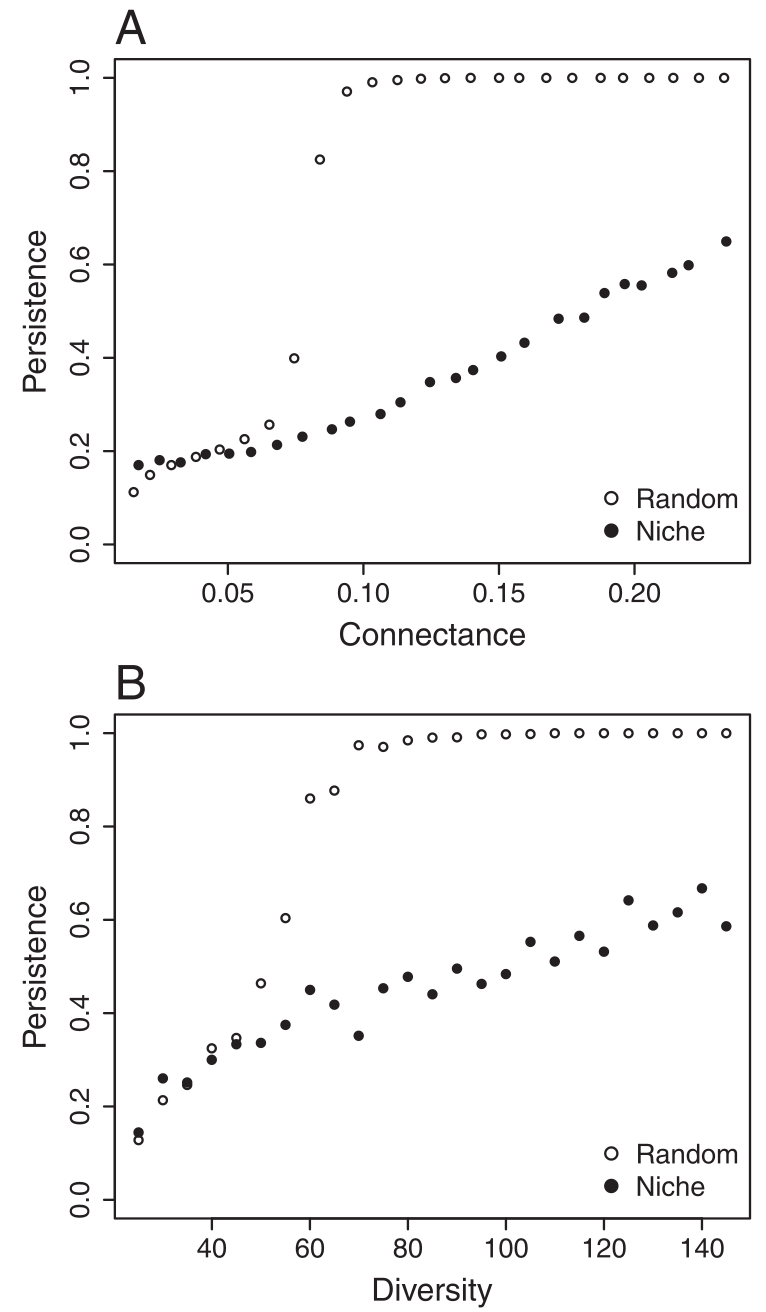
\includegraphics[height=0.7\textheight]{Figs/gravel2011b}\\
        \footnotesize Gravel et al. 2011. PLOS ONE
    \end{center}

\end{frame}

%------------------------------
% IBT Exercise
%------------------------------

{
\usebackgroundtemplate{}
\begin{frame}

	\pagecolor{BDQC1st}
	\color{white}

	\LARGE{\textit{Exercise}}

\end{frame}
}

%------------------------------

\begin{frame}{Adding interactions to IBT}

    Now, using the regional food web of Havens from the github repository, explores the species-area relationships of the different trophic levels. 

    The basic assumptions remain the same : 
    \begin{enumerate}
        \item A species can only invade an island if it as at least one prey present on the island
        \item A species that loses its last prey on the island goes extinct
    \end{enumerate}

    Implicit assumption : species with no prey in the metaweb are primary producers and therefore do not require prey to persist.

\end{frame}

%------------------------------
% Trophic IBT
%------------------------------

{
\usebackgroundtemplate{}
\begin{frame}

	\pagecolor{BDQC1st}
	\color{white}

	\LARGE{\textit{Trophic Island Biogeography}}

\end{frame}
}

%------------------------------

\begin{frame}{Island interaction networks}
	\begin{columns}
		\begin{column}{0.6\textwidth}	
			\begin{center}
				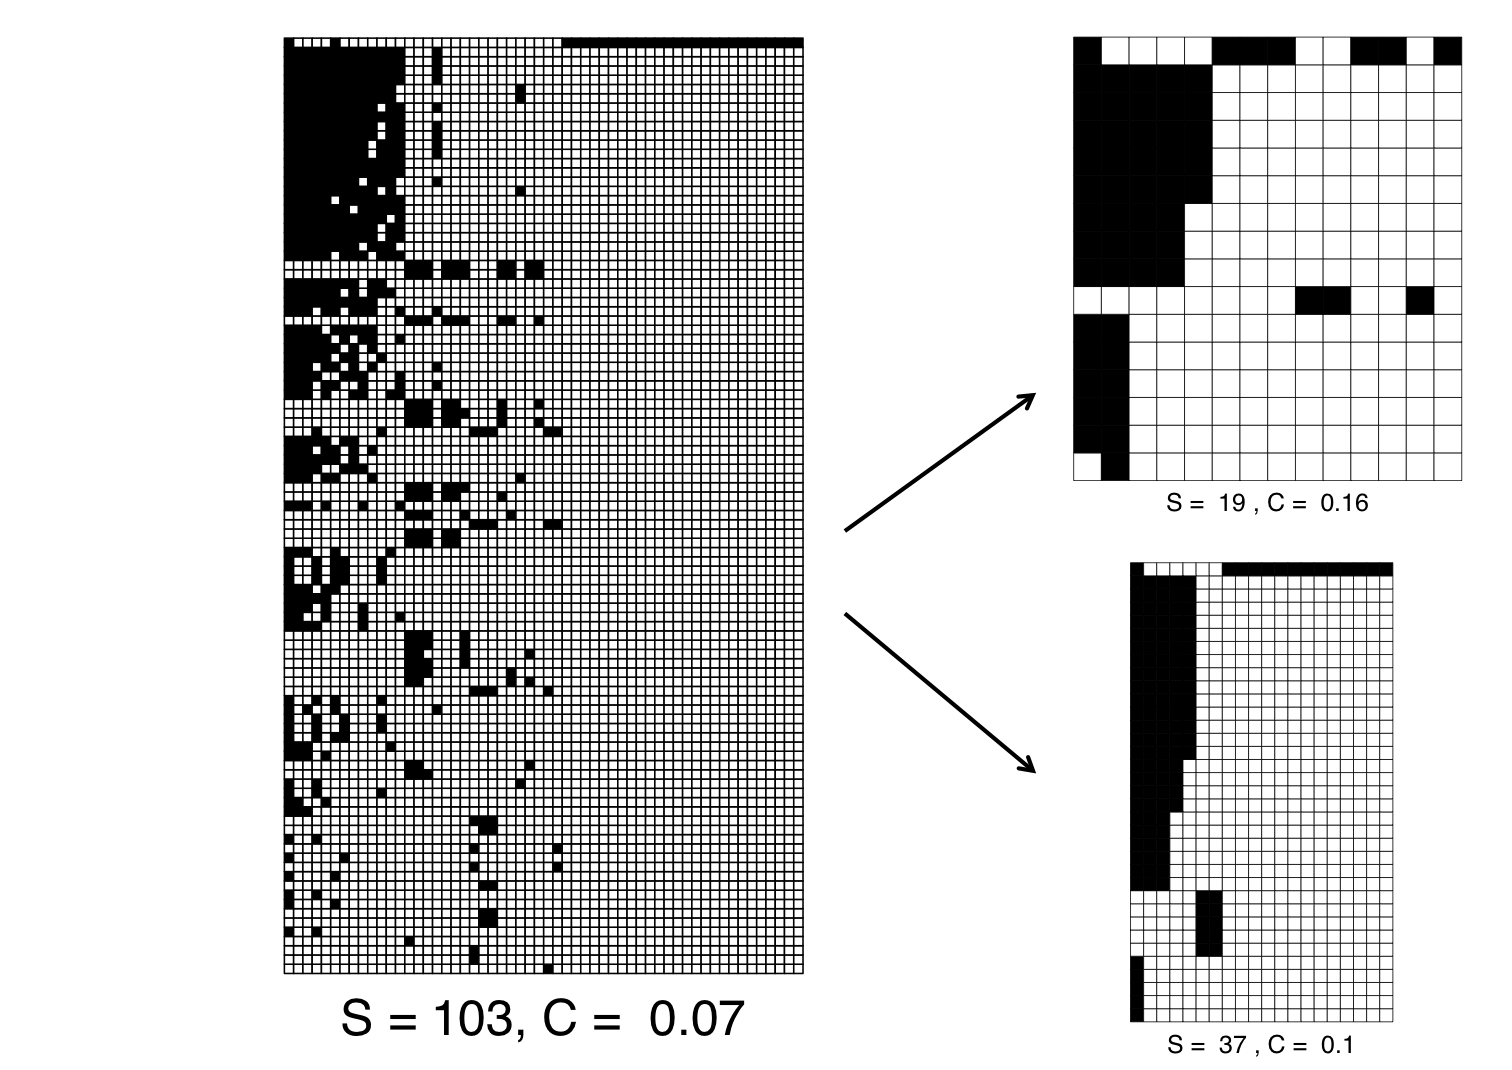
\includegraphics[height=0.6\textheight]{Figs/mw_sampling}\\	
			\end{center}  
		\end{column}
%----
		\begin{column}{0.4\textwidth}			
			Comparison to the regional pool : 
			\begin{itemize}
				\item Larger number of links
				\item Larger connectance
				\item Shorter food chains
				\item Fully connected network
			\end{itemize}  			
		\end{column}				
	\end{columns} 		
	\vskip 1em
\end{frame}

%------------------------------

\begin{frame}{Trophic IBT}{Model}

    \textbf{Assumptions:}	\\
 
    \begin{itemize}
        \item A species can only invade an island if it as at least one prey present 
        on the island
        \item A species that loses its last prey on the island goes extinct
    \end{itemize}

    \begin{columns}
        \begin{column}{0.5\textwidth}			

            \keyeqs{\frac{dp_g}{dt} =	 c(1-p_g)q_g - (e + \epsilon_g)p_g}

            where:\\

            \keyeqs{p^*_g = \frac{cq_g}{cq_g + e + \epsilon_g}}

        \end{column}
    %----
        \begin{column}{0.5\textwidth}
            \begin{itemize}
                \item $c$: colonization rate
                \item $e$: community-independent extinction rate
                \item $q_g$: probability that a species has a prey present on the island
                \item $\epsilon_g$: rate a predator loses its last prey on the island
            \end{itemize}
        \end{column}
    \end{columns}	    

\end{frame}


\begin{frame}{Equilibrium species richness}
	    
    \begin{center}
        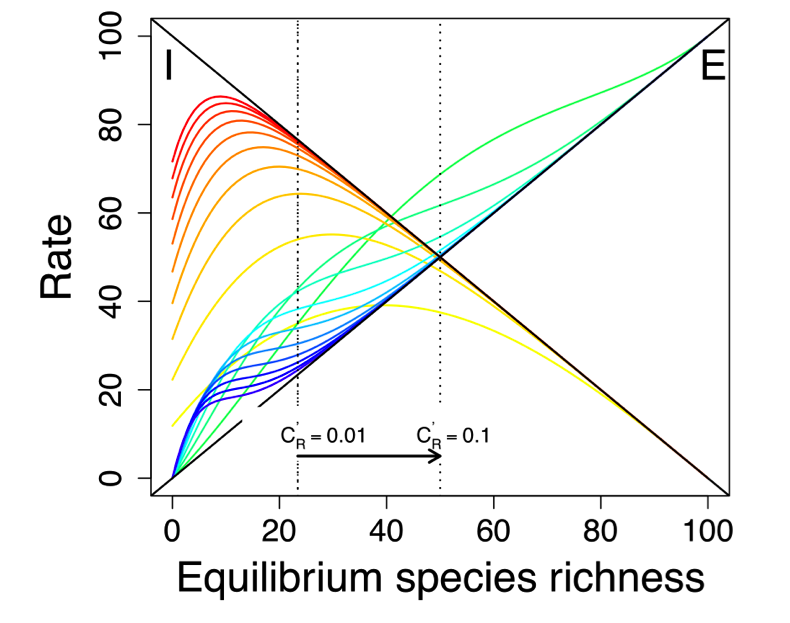
\includegraphics[height=0.65\textheight]{Figs/ttib}\\
        \footnotesize{Gravel et al. (2011) \textit{Ecology Letters}.}
    \end{center}
\end{frame}

%------------------------------

\begin{frame}{Network assembly dynamics}
    
    \begin{center}
        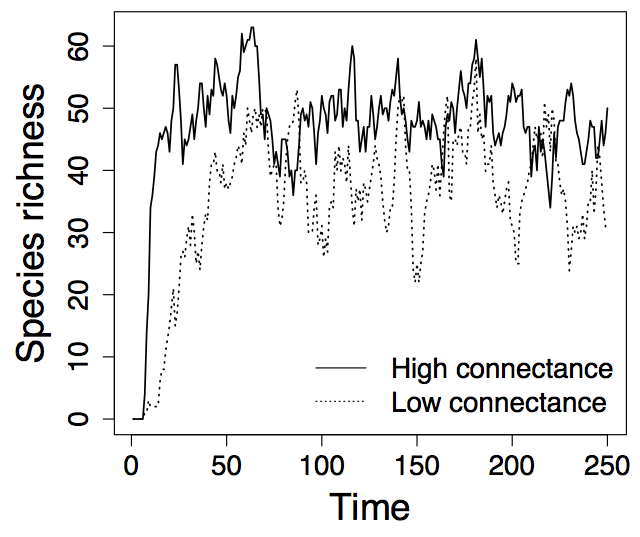
\includegraphics[height=0.65\textheight]{Figs/ttib_dynamics}\\
        \footnotesize{Gravel et al. (2011) \textit{Ecology Letters}.}
    \end{center}

\end{frame}

%------------------------------

\begin{frame}{Local-regional feedback}
    
    \begin{columns}
        \begin{column}{0.5\textwidth}			
            \begin{center}
                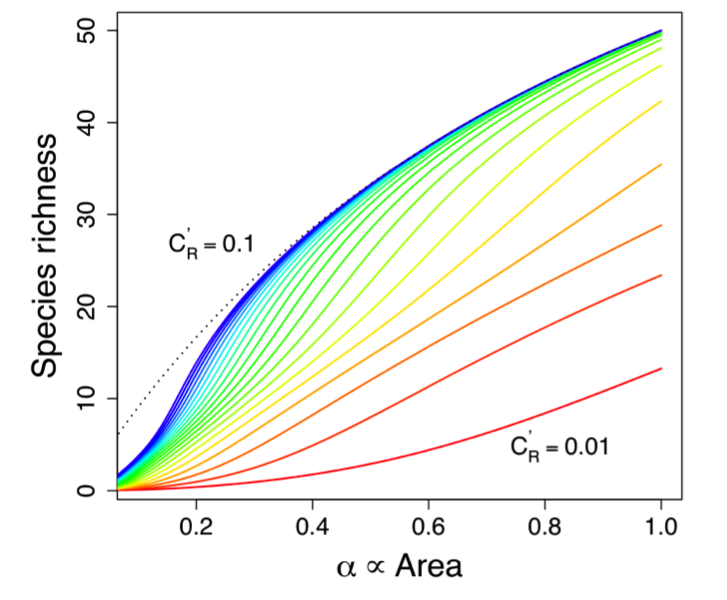
\includegraphics[height=0.5\textheight]{Figs/trophicSAR}\\
            \end{center}

        \end{column}
%----
        \begin{column}{0.5\textwidth}
            \begin{center}
                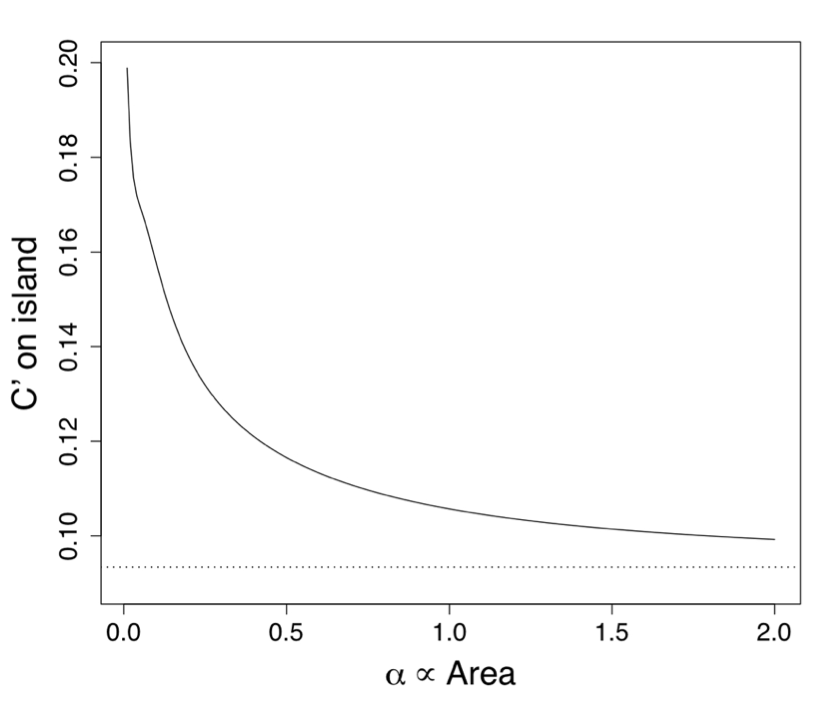
\includegraphics[height=0.5\textheight]{Figs/connectance_area}\\
            \end{center}
        \end{column}
           
    \end{columns}	   

\end{frame}

%------------------------------

\begin{frame}{Testing theory}{Species distribution}
    
    \begin{columns}
        \begin{column}{0.4\textwidth}			
            \begin{center}
                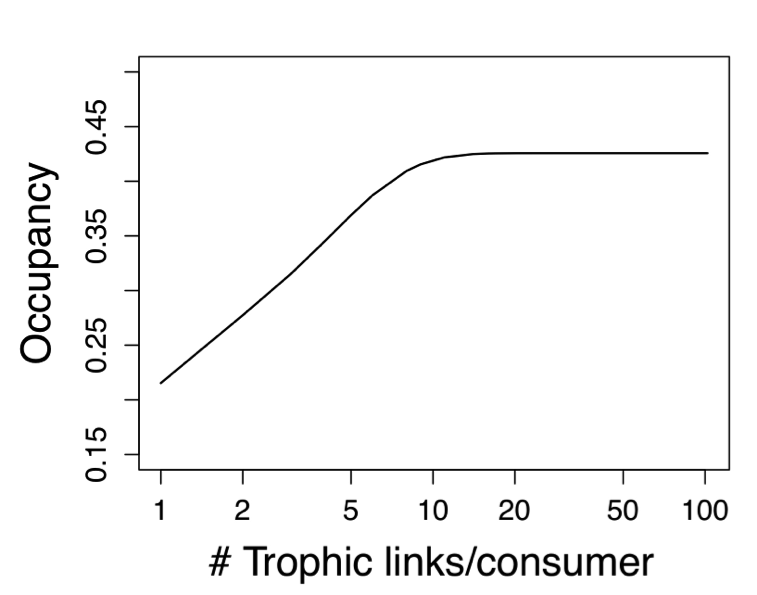
\includegraphics[height=0.45\textheight]{Figs/occupancy}\\
            \end{center}

        \end{column}
%----
        \begin{column}{0.6\textwidth}
            \begin{center}
                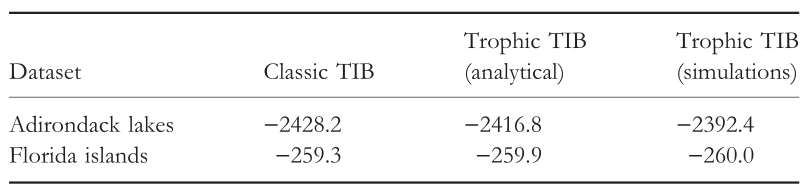
\includegraphics[height=0.2\textheight]{Figs/gravel2011c}\\
            \end{center}
        \end{column}
           
    \end{columns}	   

\end{frame}

%------------------------------

\begin{frame}{Testing theory}{Scaling relationships}
    
    \begin{center}
        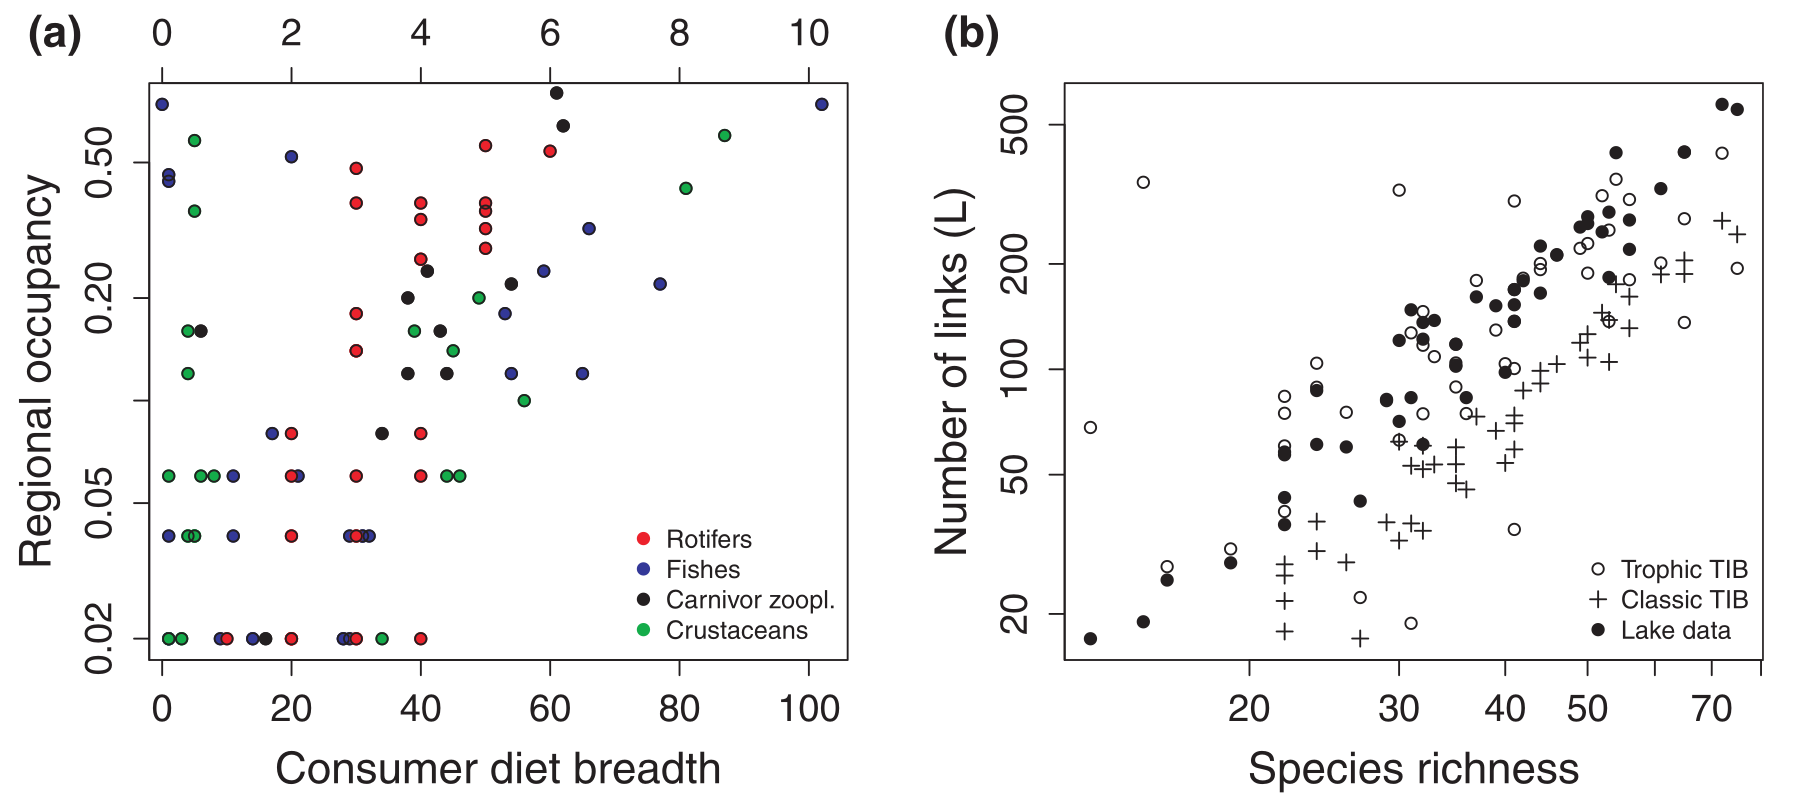
\includegraphics[height=0.6\textheight]{Figs/gravel2011d}\\
        \footnotesize{Gravel et al. (2011) \textit{Ecology Letters}.}
    \end{center}

\end{frame}

%------------------------------
% Trait-based IBT
%------------------------------

{
\usebackgroundtemplate{}
\begin{frame}

	\pagecolor{BDQC1st}
	\color{white}

	\LARGE{\textit{Trait-based IBT}}

\end{frame}
}

%------------------------------

\begin{frame}{The mass-area relationship}
	
	\begin{center}
		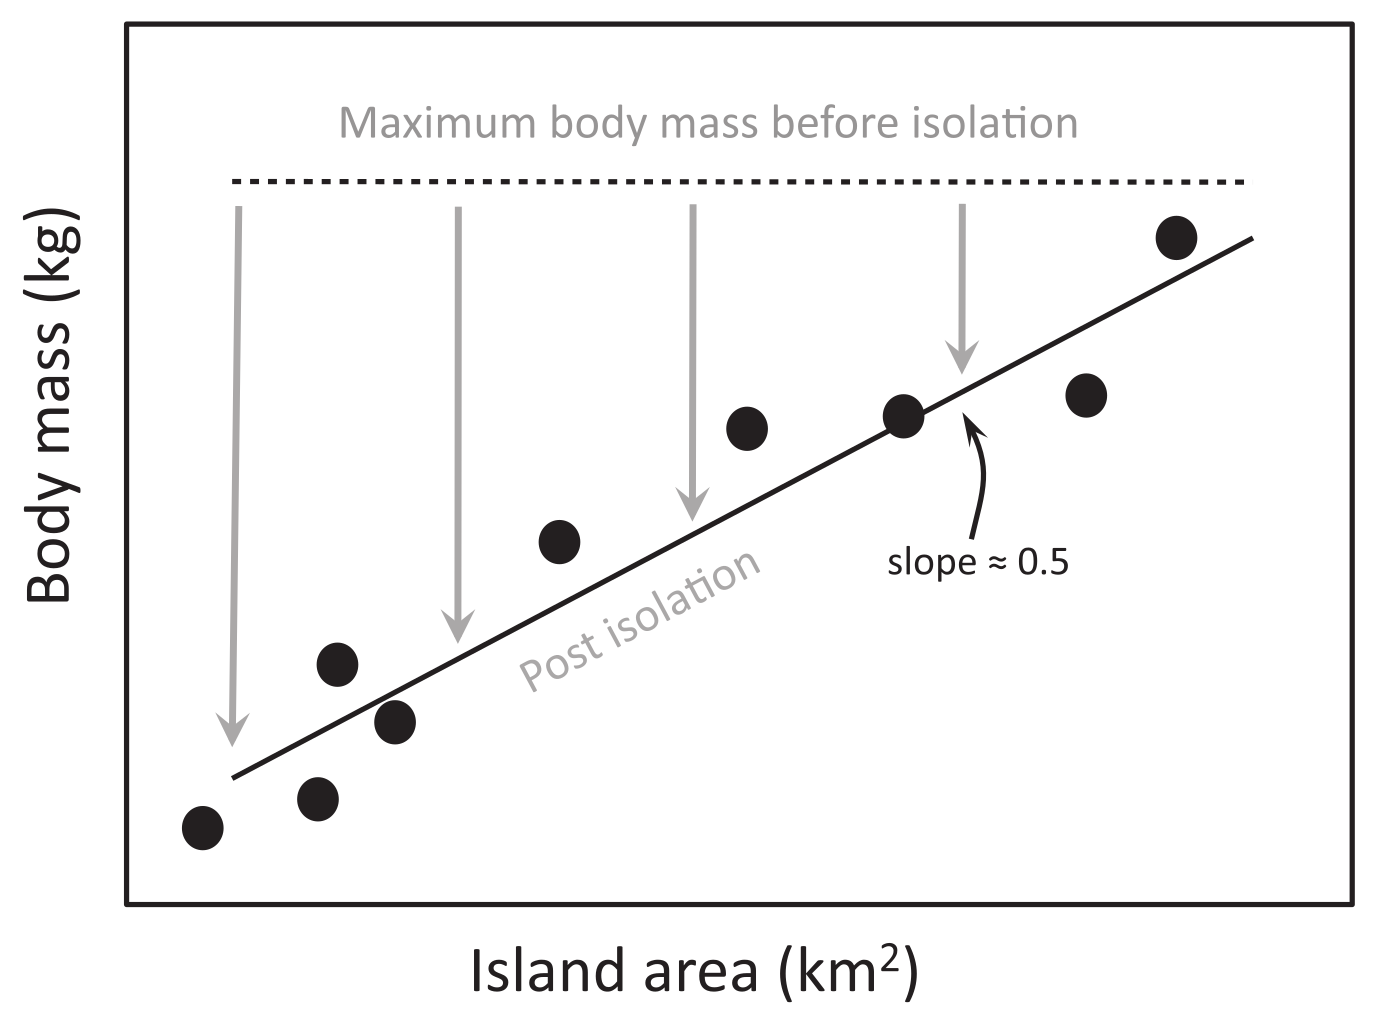
\includegraphics[height=0.65\textheight]{Figs/millien2011a}\\ % TODO: image missing from Figs/
		\footnotesize{Millien and Gonzalez (2011) J. Biogeo}
	\end{center}

\end{frame}

% %------------------------------

\begin{frame}{Body-size and insular dynamics}
	\begin{columns}
		\begin{column}{0.6\textwidth}	
			\begin{center}
				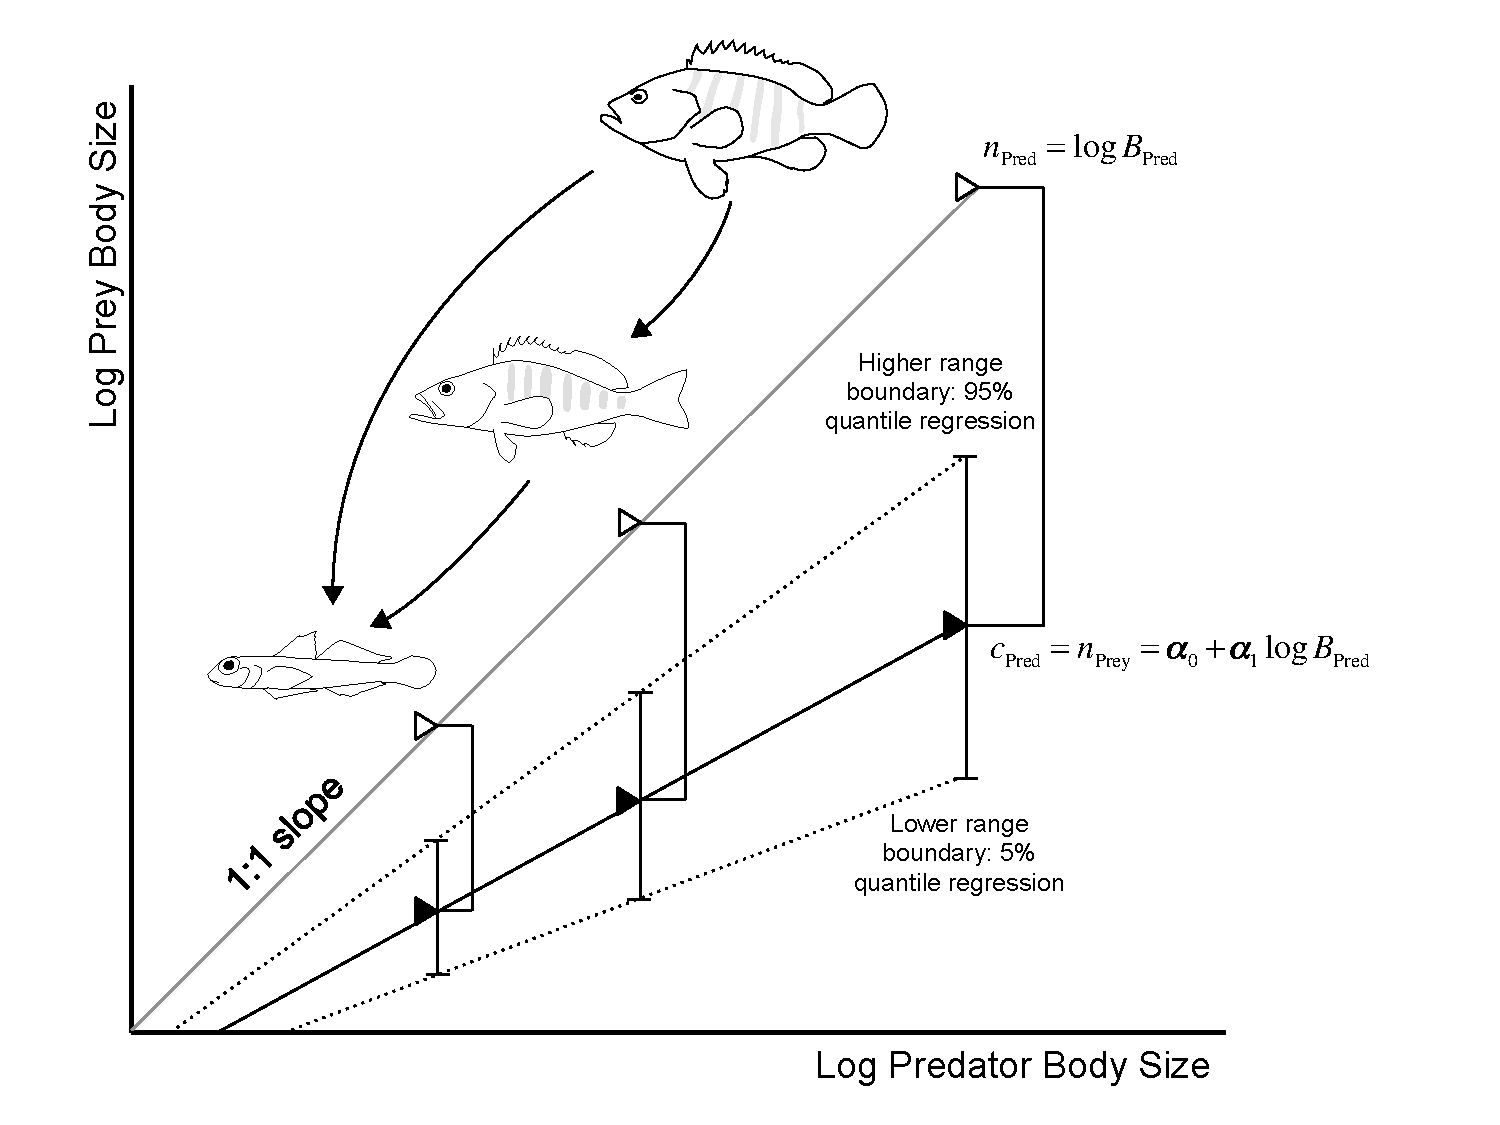
\includegraphics[height=0.6\textheight]{Figs/gravel2012}\\	
			\end{center}  
		\end{column}
%----
		\begin{column}{0.4\textwidth}			
			\begin{itemize}
				\item Dispersal distance 
				\item Number of propagules
				\item Energetic requirements
				\item Home range
				\item Population size
				\item Trophic level
				\item Diet breadth
				\item [....]
			\end{itemize}	
		\end{column}				
	\end{columns} 	
\end{frame}

%------------------------------

\begin{frame}{Body-size and insular dynamics}
	\begin{columns}
		\begin{column}{0.6\textwidth}	
			\begin{center}
				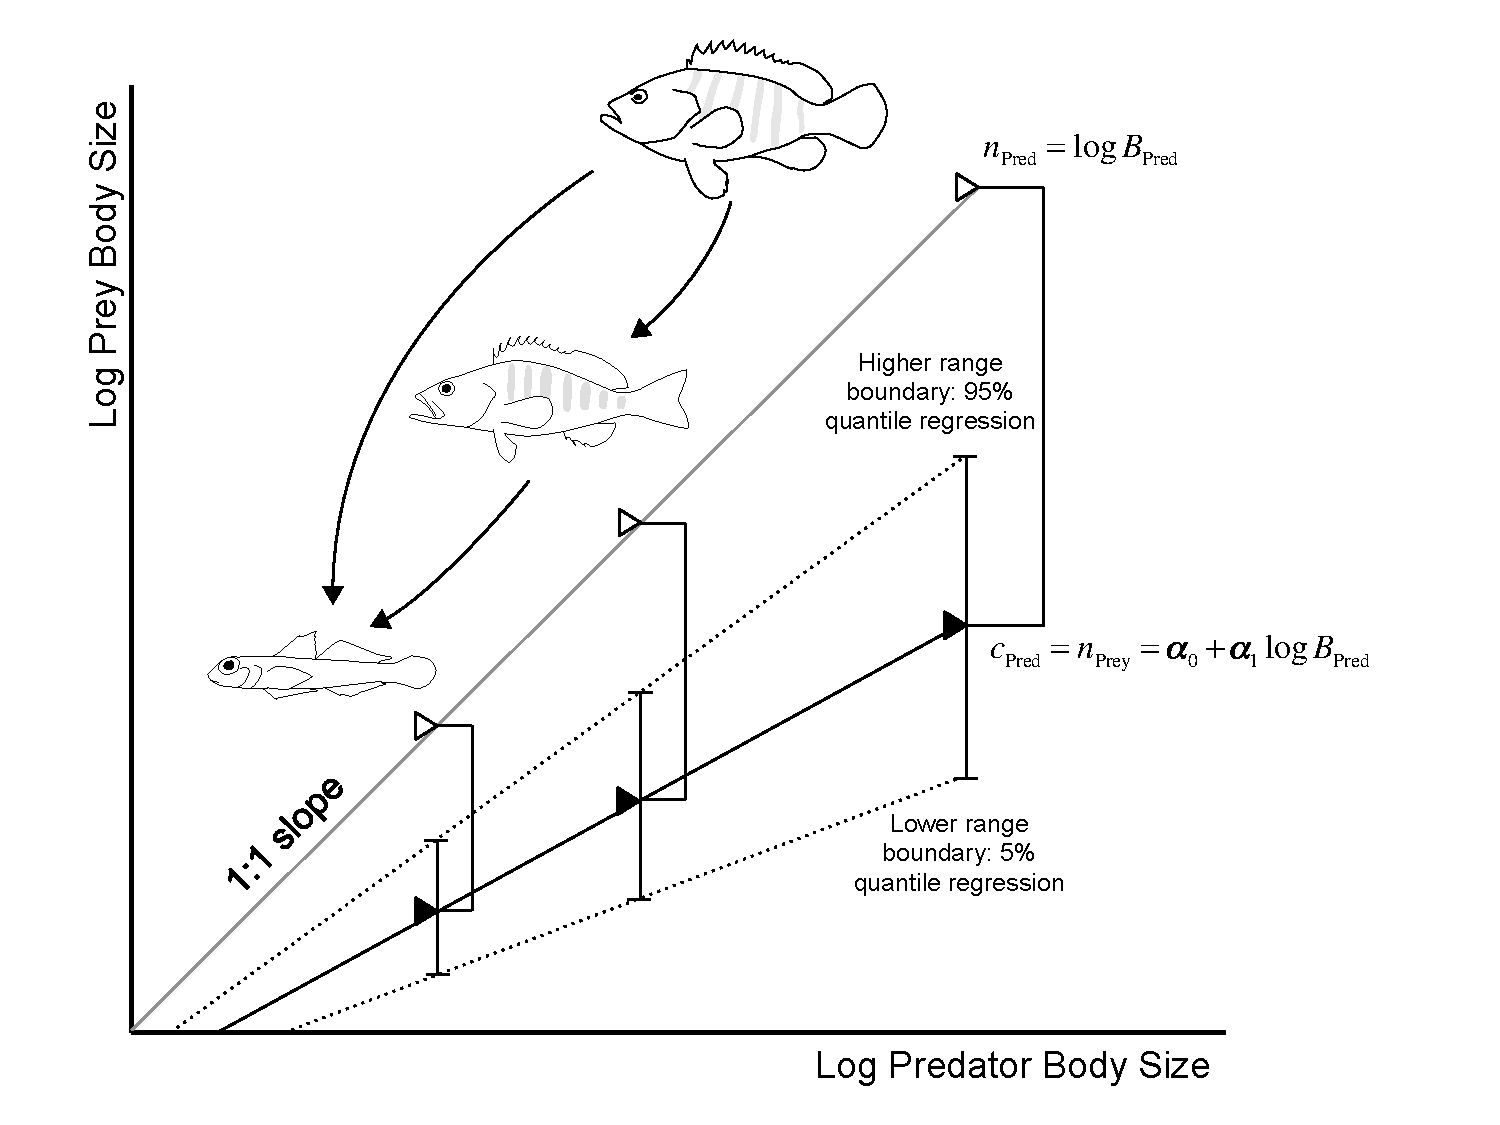
\includegraphics[height=0.6\textheight]{Figs/gravel2012}\\	
			\end{center}  
		\end{column}
%----
		\begin{column}{0.4\textwidth}			
		Additions to the model : 
			\begin{itemize}
				\item Size-constraint food web
				\item Size-dependent $c$ and $e$ parameters
			\end{itemize}	
		\end{column}				
	\end{columns} 	
\end{frame}

%------------------------------

\begin{frame}{Islands as a non-random sample from the regional pool}

	\begin{center}
		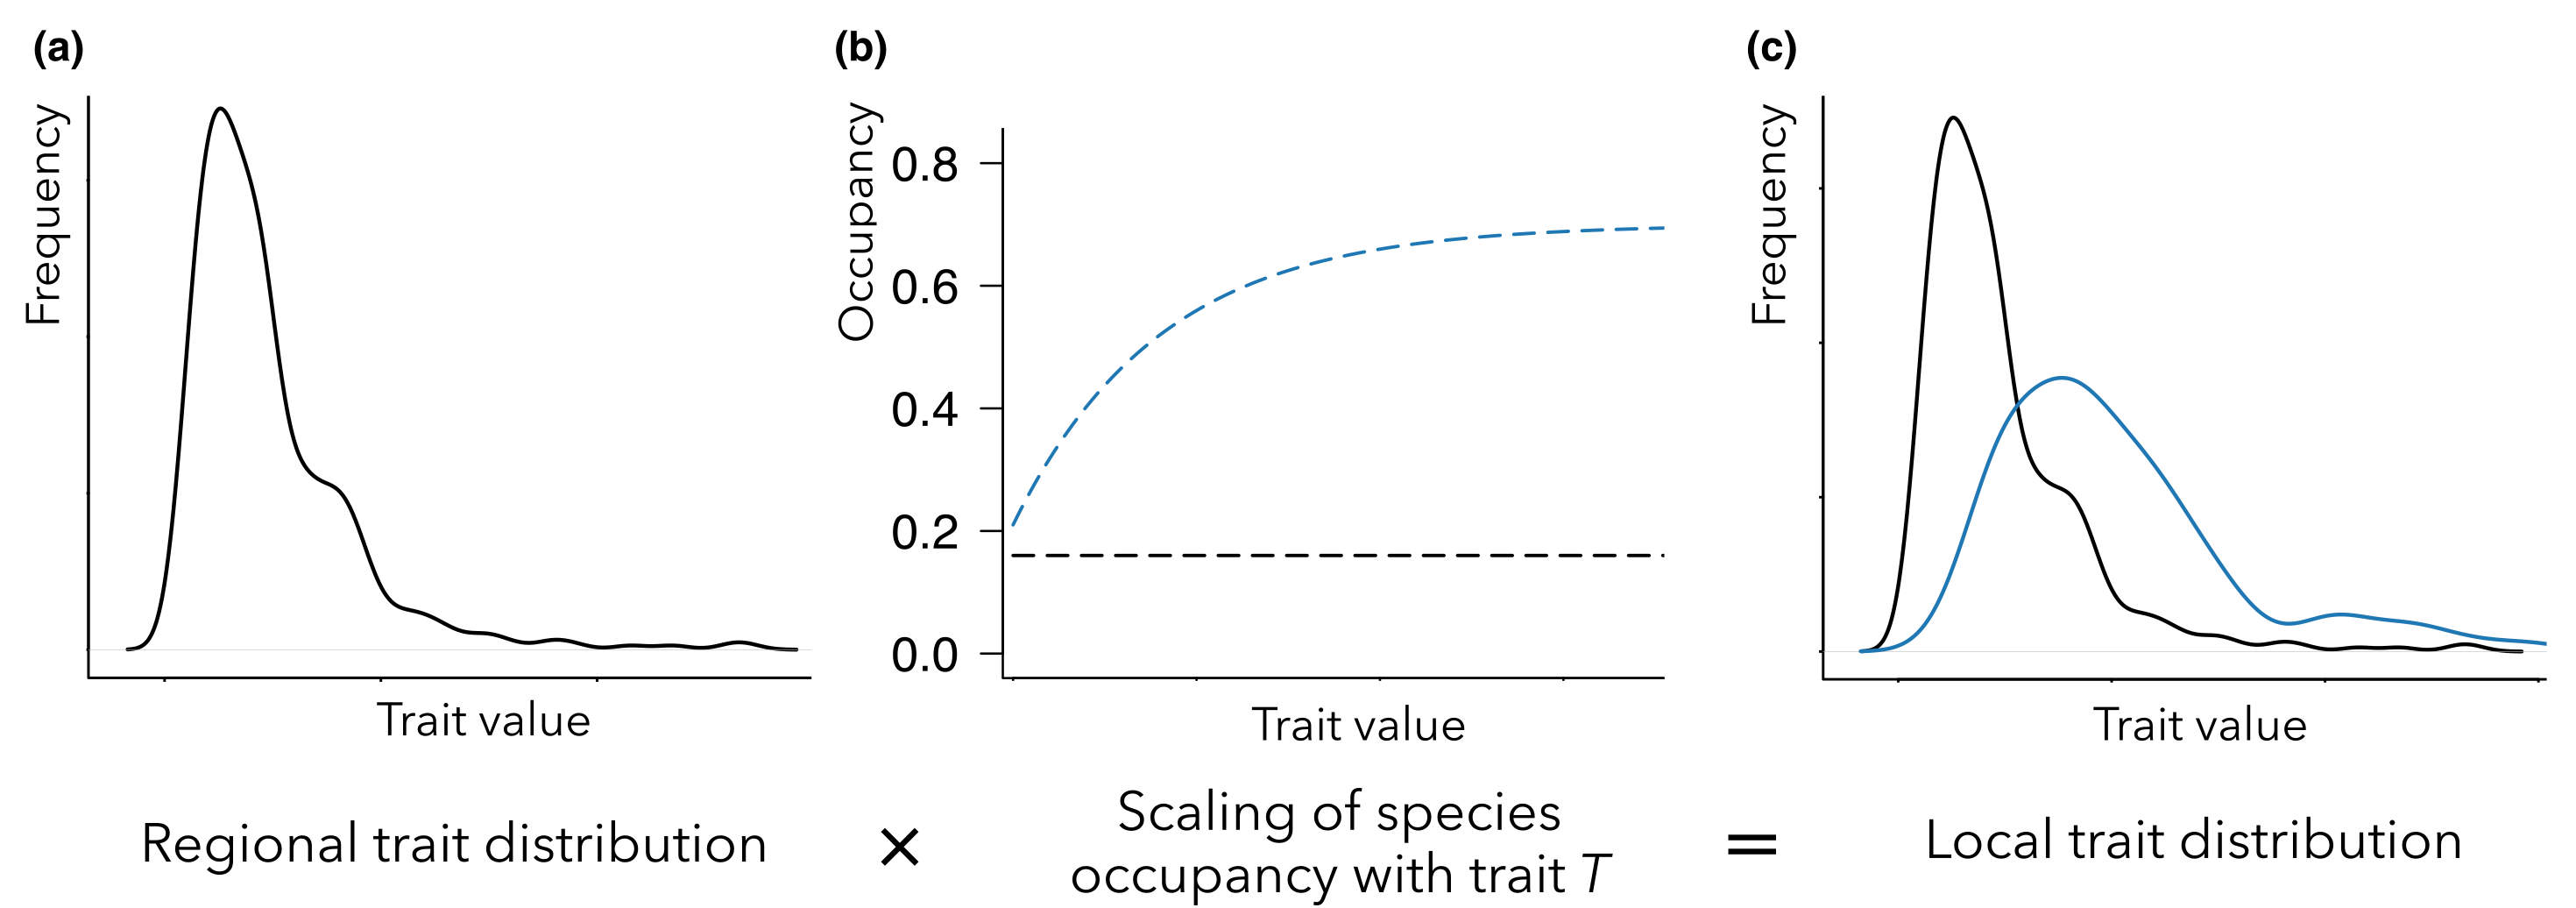
\includegraphics[height=0.5\textheight]{Figs/jacquet2017a}\\	
		\vskip 1em
		\footnotesize{Jacquet et al (2017) Ecol. Lett.}
	\end{center}  

\end{frame}

%------------------------------

\begin{frame}{Size distribution in coral reefs}
	\begin{columns}
		\begin{column}{0.4\textwidth}			
			\textbf{Expectations :}
			\begin{itemize}
				\item Variance in body-size increases (decreases) with area (isolation) for resources
				\item Variance in body-size decreases (decreases) with area (isolation) for consumers
			\end{itemize}	
		\end{column}	
%----
		\begin{column}{0.6\textwidth}	
			\begin{center}
				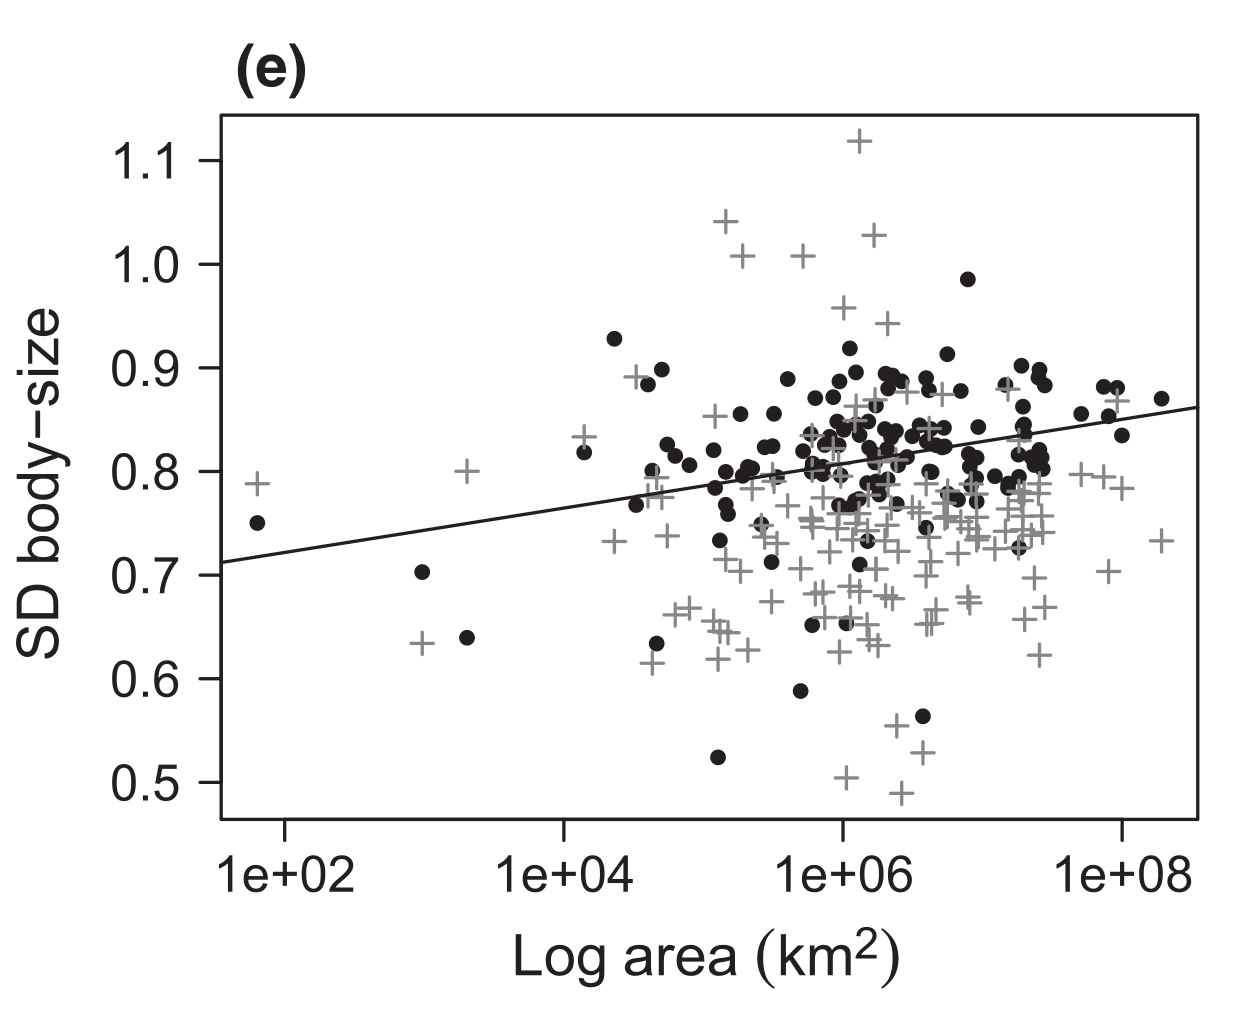
\includegraphics[height=0.6\textheight]{Figs/jacquet2017b}\\	
				\footnotesize{Jacquet et al (2017) Ecol. Lett.}
			\end{center}  
		\end{column}			
	\end{columns} 	
\end{frame}

%------------------------------
% Macro-evolution
%------------------------------

{
\usebackgroundtemplate{}
\begin{frame}

	\pagecolor{BDQC1st}
	\color{white}

	\LARGE{\textit{And macro-evolution}}

\end{frame}
}

%------------------------------

\begin{frame}{Trait-matching concept}
	\begin{columns}
		\begin{column}{0.6\textwidth}	
			\begin{center}
				
\includegraphics[height=0.65\textheight]{Figs/gravel2016}\\	
				\footnotesize{Gravel et al (2016) Phil. Trans. Roy. Soc.}				
			\end{center}  
		\end{column}
%----
		\begin{column}{0.4\textwidth}			
			\begin{itemize}
				\item Network structure is the joint result of \textbf{trait-matching} and \textbf{trait-distribution}
				\item Traits could either evolve \textbf{neutrally} or under \textbf{biotic selection}
			\end{itemize}		
		\end{column}				
	\end{columns} 	
\end{frame}

%------------------------------

\begin{frame}{Trait evolution under biotic selection}
	\begin{columns}
		\begin{column}{0.55\textwidth}	
			\begin{center}
				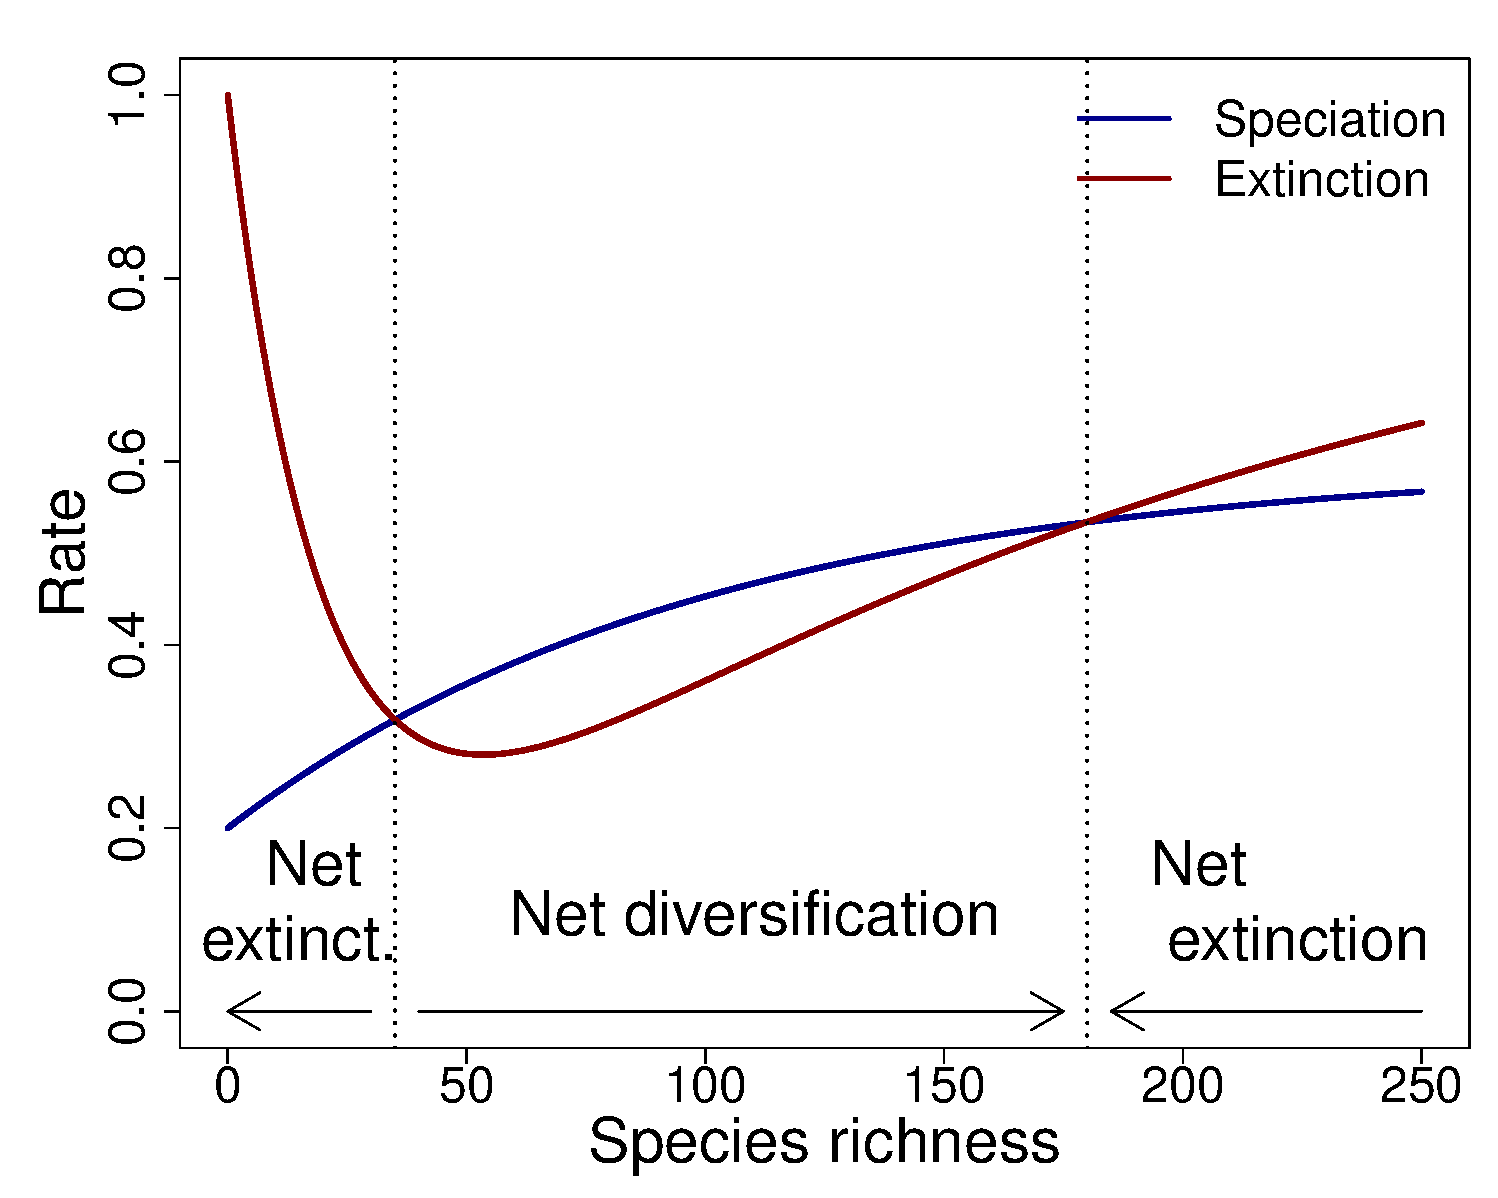
\includegraphics[height=0.6\textheight]{Figs/diversification}\\	
			\end{center}  
		\end{column}
%----
		\begin{column}{0.45\textwidth}			
		Additions to the model : 
			\begin{itemize}
				\item Trait evolution at speciation
				\item Per species constant speciation rate
				\item Establishment contingent on prey availability
				\item Top-down effect on extinction 	
				\item Tracking of phylogeny, trait distribution and pairwise interactions
			\end{itemize}  
		\end{column}				
	\end{columns} 	
\end{frame}

%------------------------------

\begin{frame}{Trait evolution under biotic selection}
	\begin{columns}
		\begin{column}{0.55\textwidth}	
			\begin{center}
				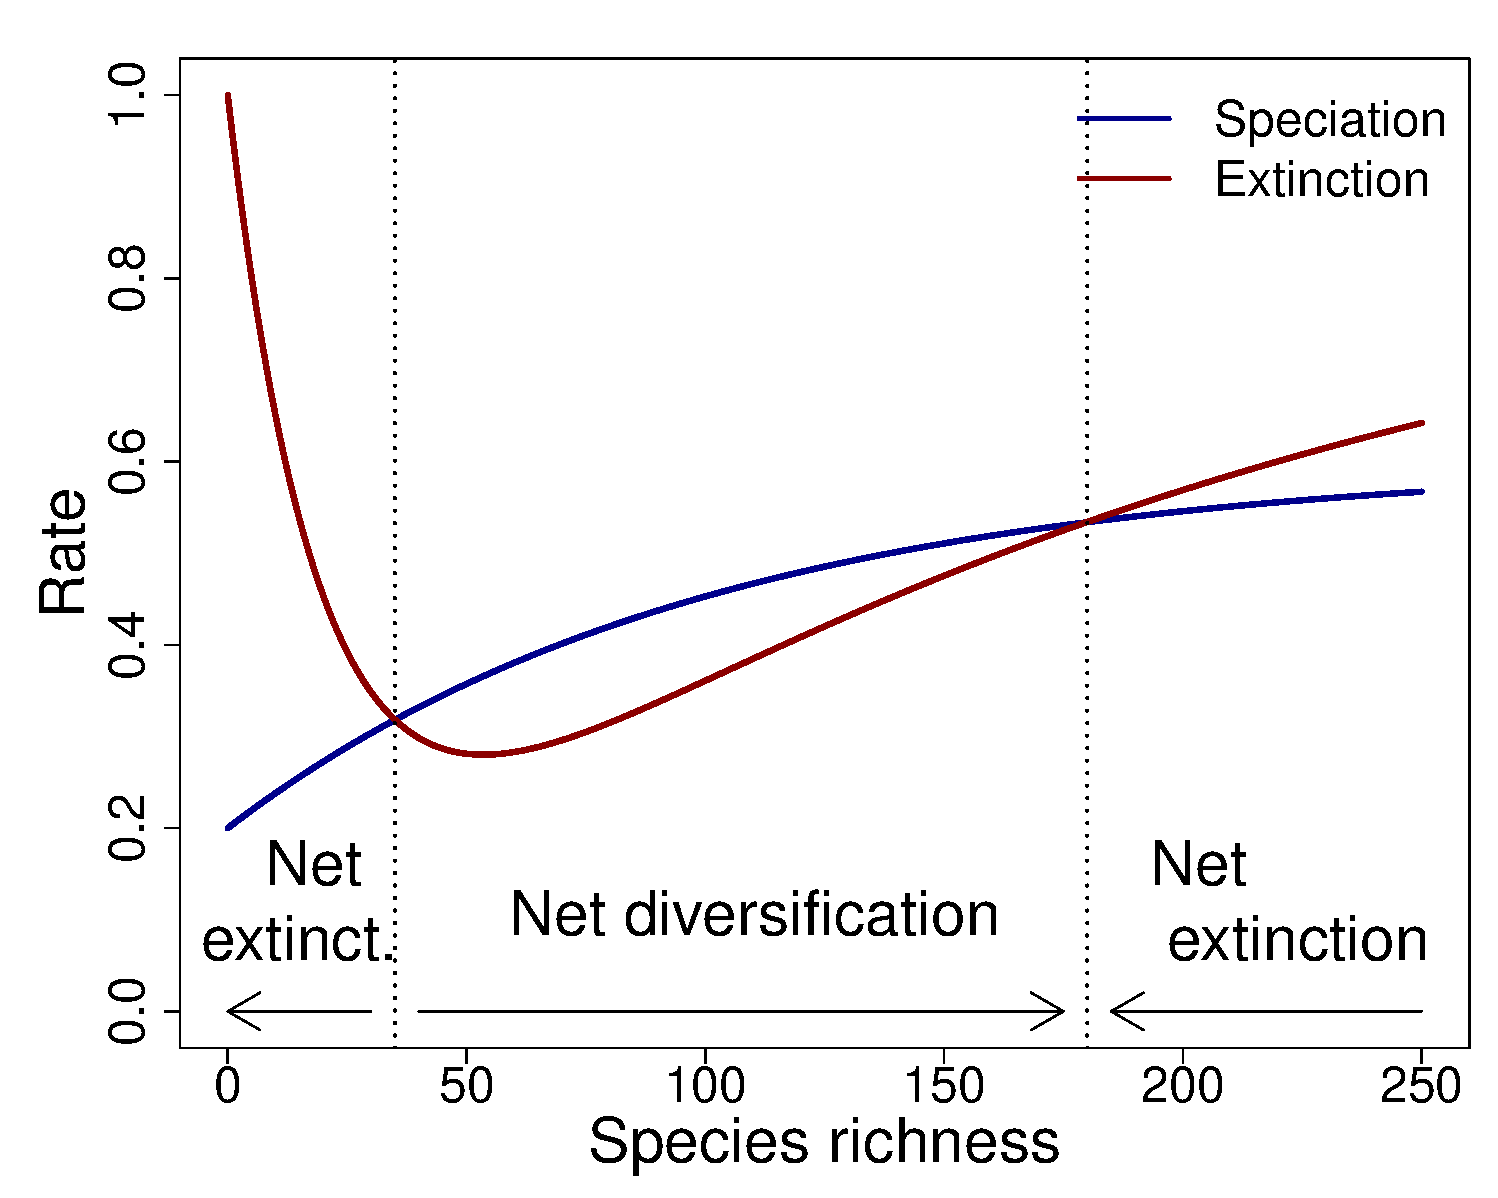
\includegraphics[height=0.6\textheight]{Figs/diversification}\\	
			\end{center}  
		\end{column}
%----
		\begin{column}{0.45\textwidth}			
			\begin{center}
				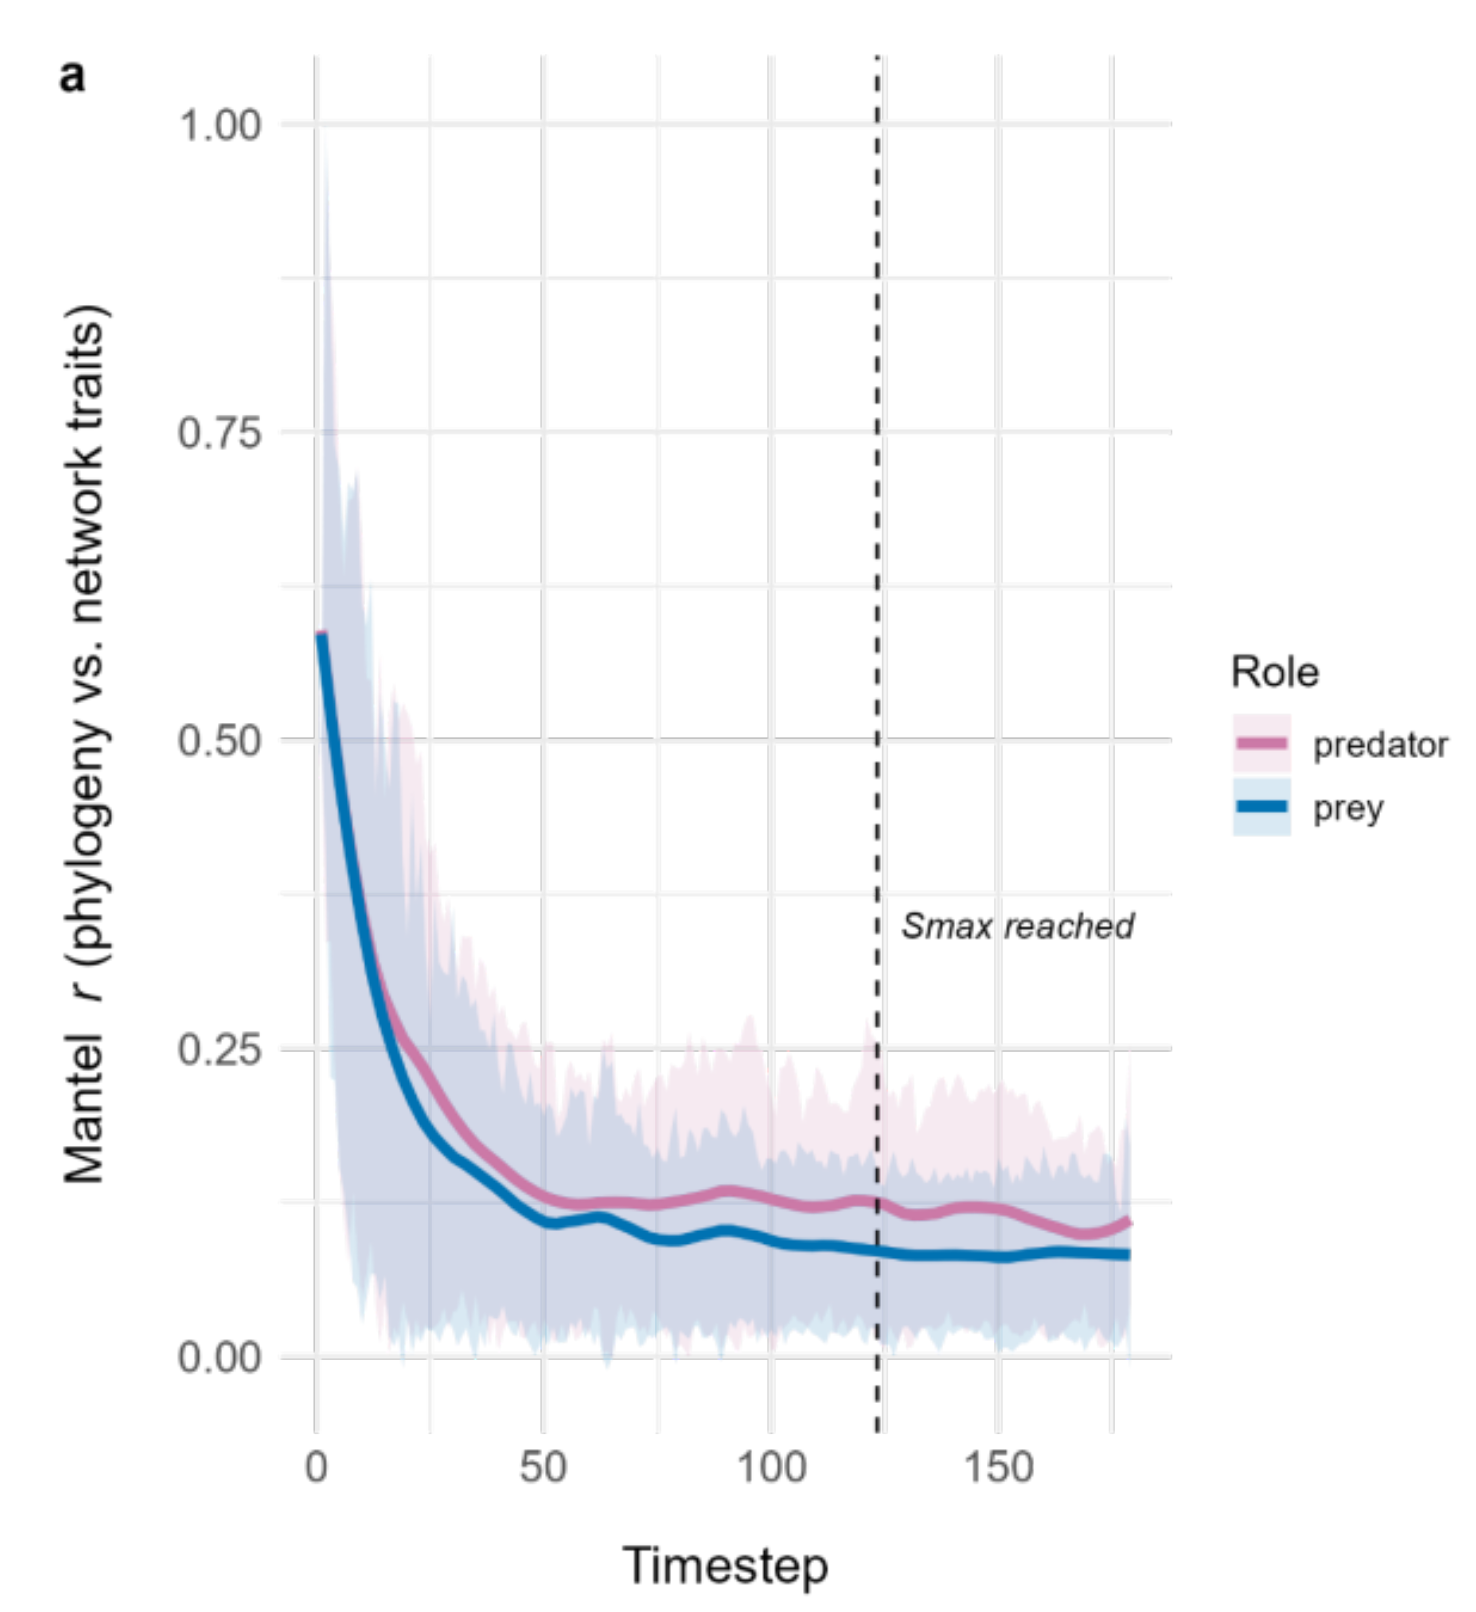
\includegraphics[height=0.7\textheight]{Figs/fuster2025a}\\	
			\end{center}  
		\end{column}				
	\end{columns} 	
\end{frame}

%------------------------------

\begin{frame}{Phylogenetic signal in Galapagos food webs}
	\begin{columns}
		\begin{column}{0.6\textwidth}	
			\begin{center}
				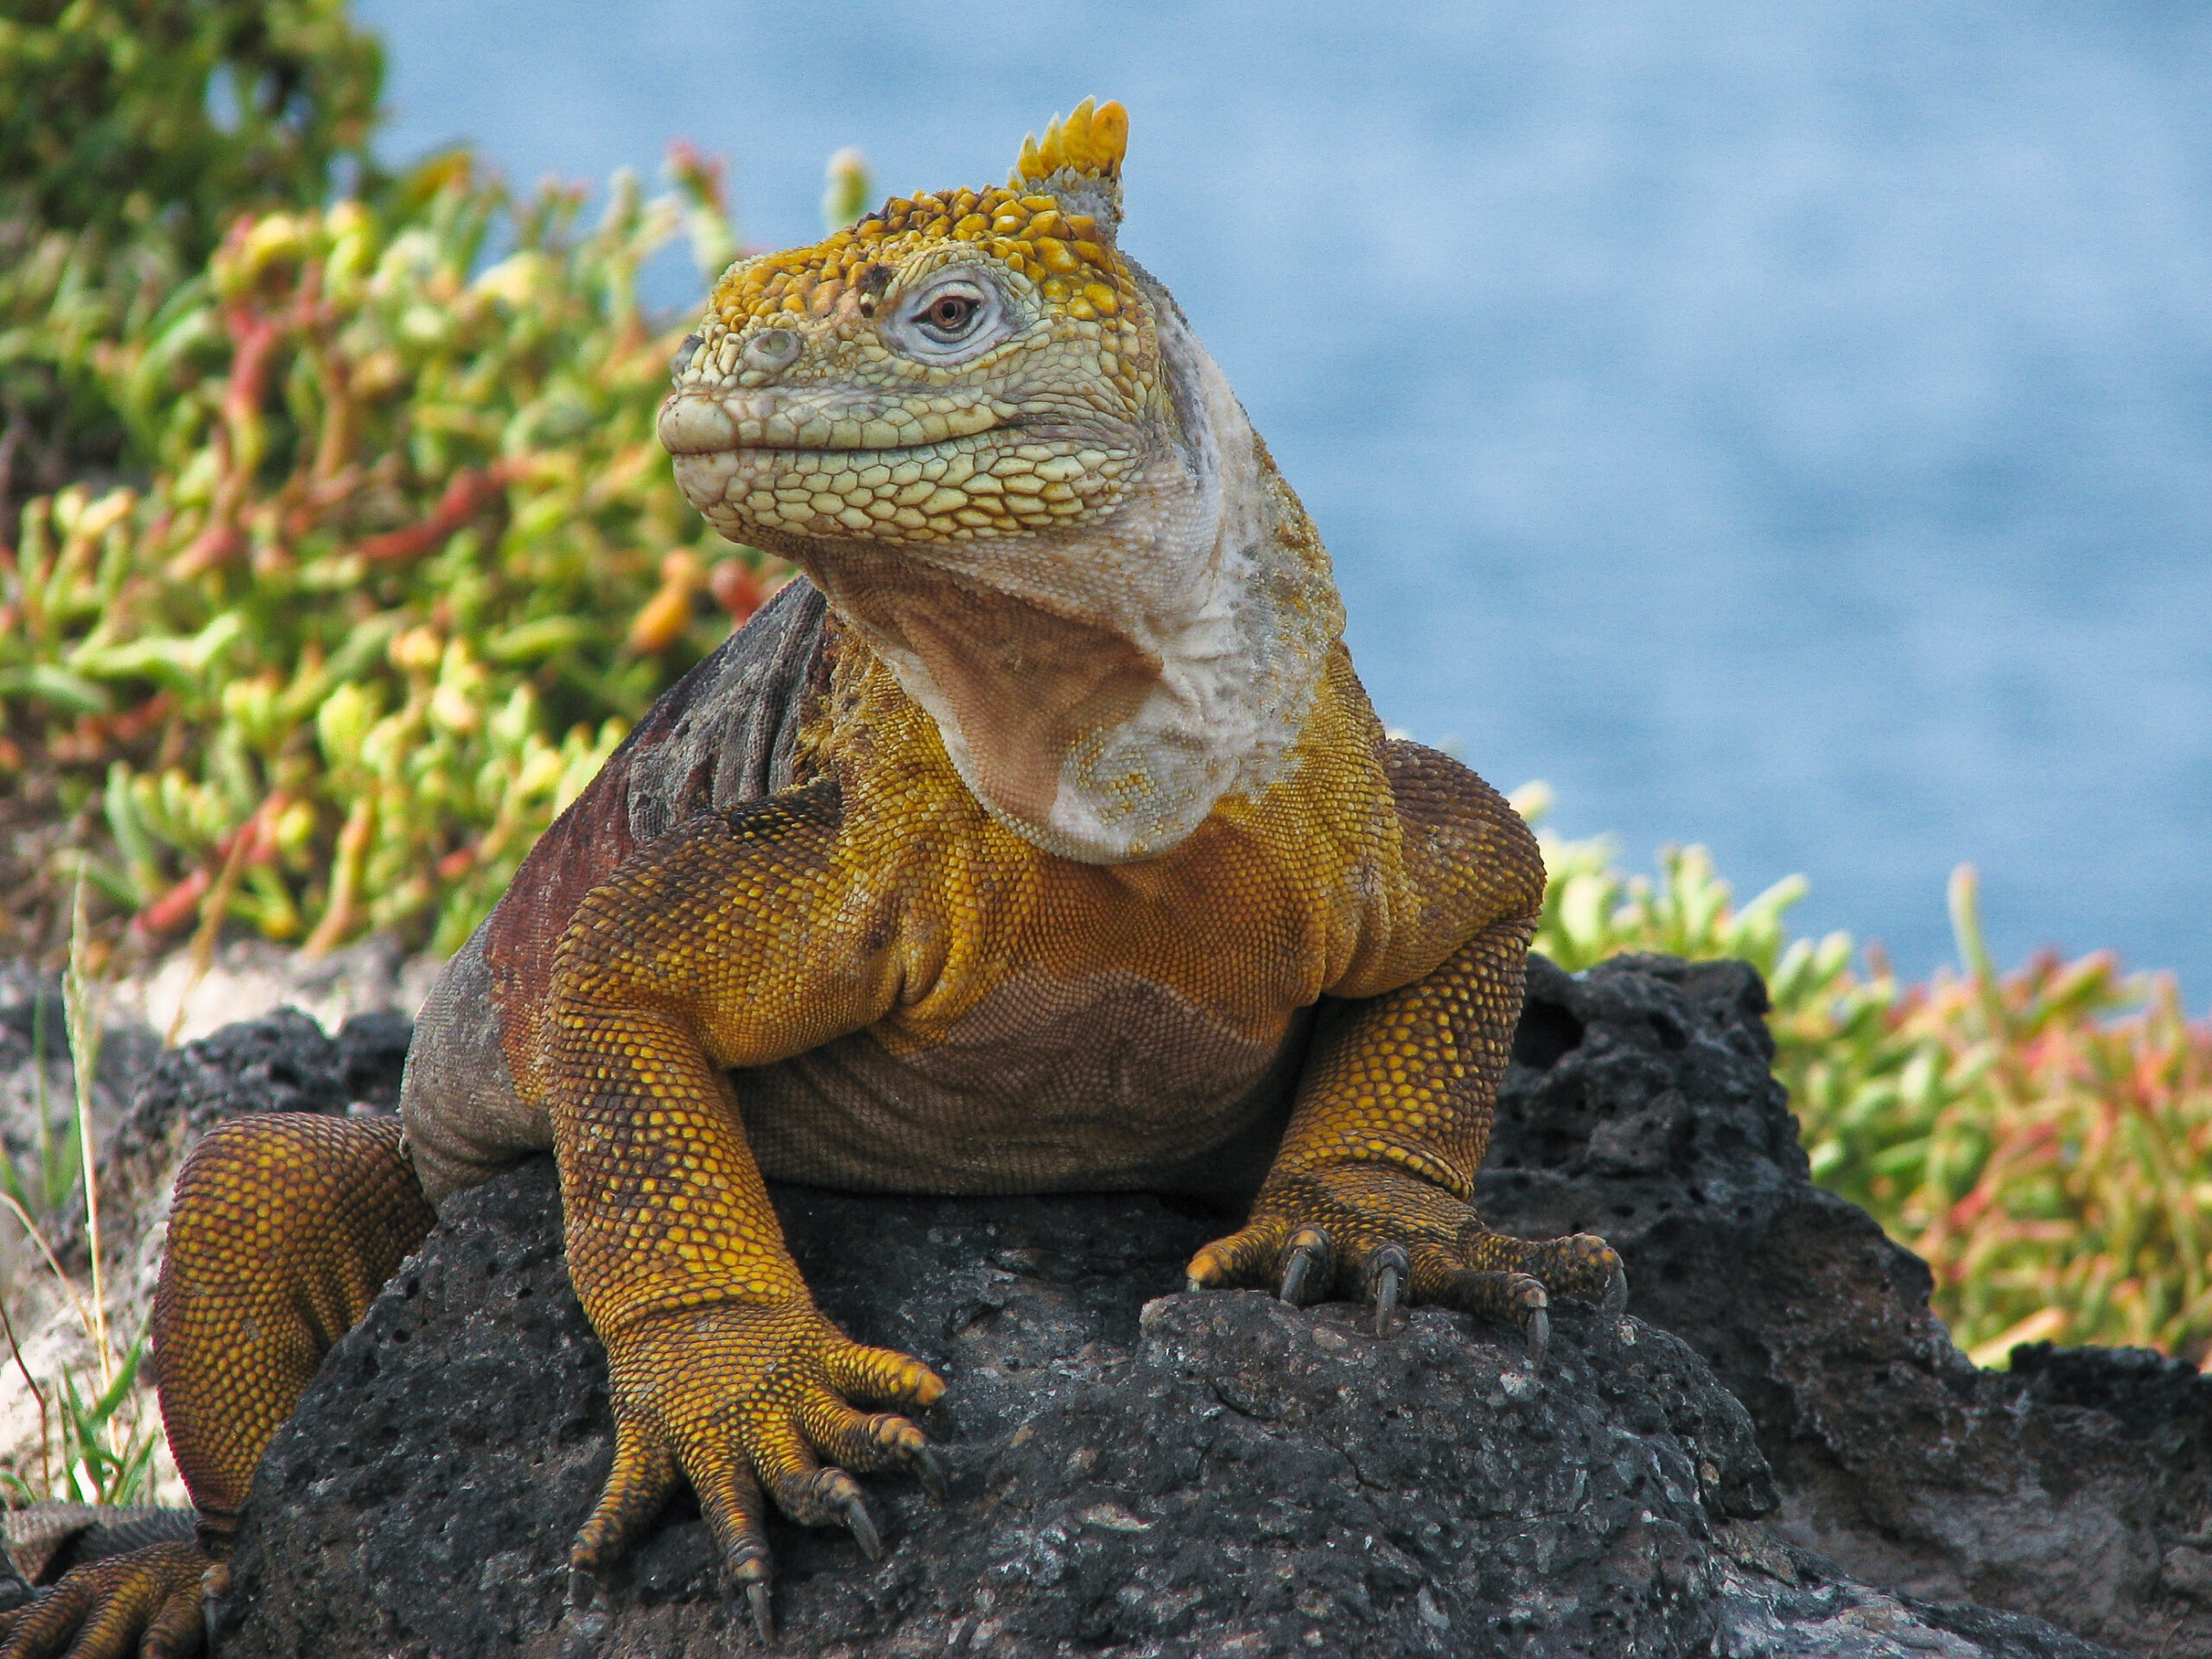
\includegraphics[height=0.55\textheight]{Figs/iguana}\\	
			\end{center}  
		\end{column}
%----
		\begin{column}{0.4\textwidth}						
			\begin{itemize}
				\item Regional metaweb approach
				\item 559 species, 96 birds, 40 reptiles, 20 mammals, 402 plants, 1 invertebrate
				\item Species checklists for 13 islands of various ages
				\item Interactions from the literature
				\item 2582 links, mean trophic rank of 3.55 (metaweb)
			\end{itemize}  
		\end{column}				
	\end{columns} 	
\end{frame}

%------------------------------

\begin{frame}{Phylogenetic signal in Galapagos food webs}

	\begin{center}
		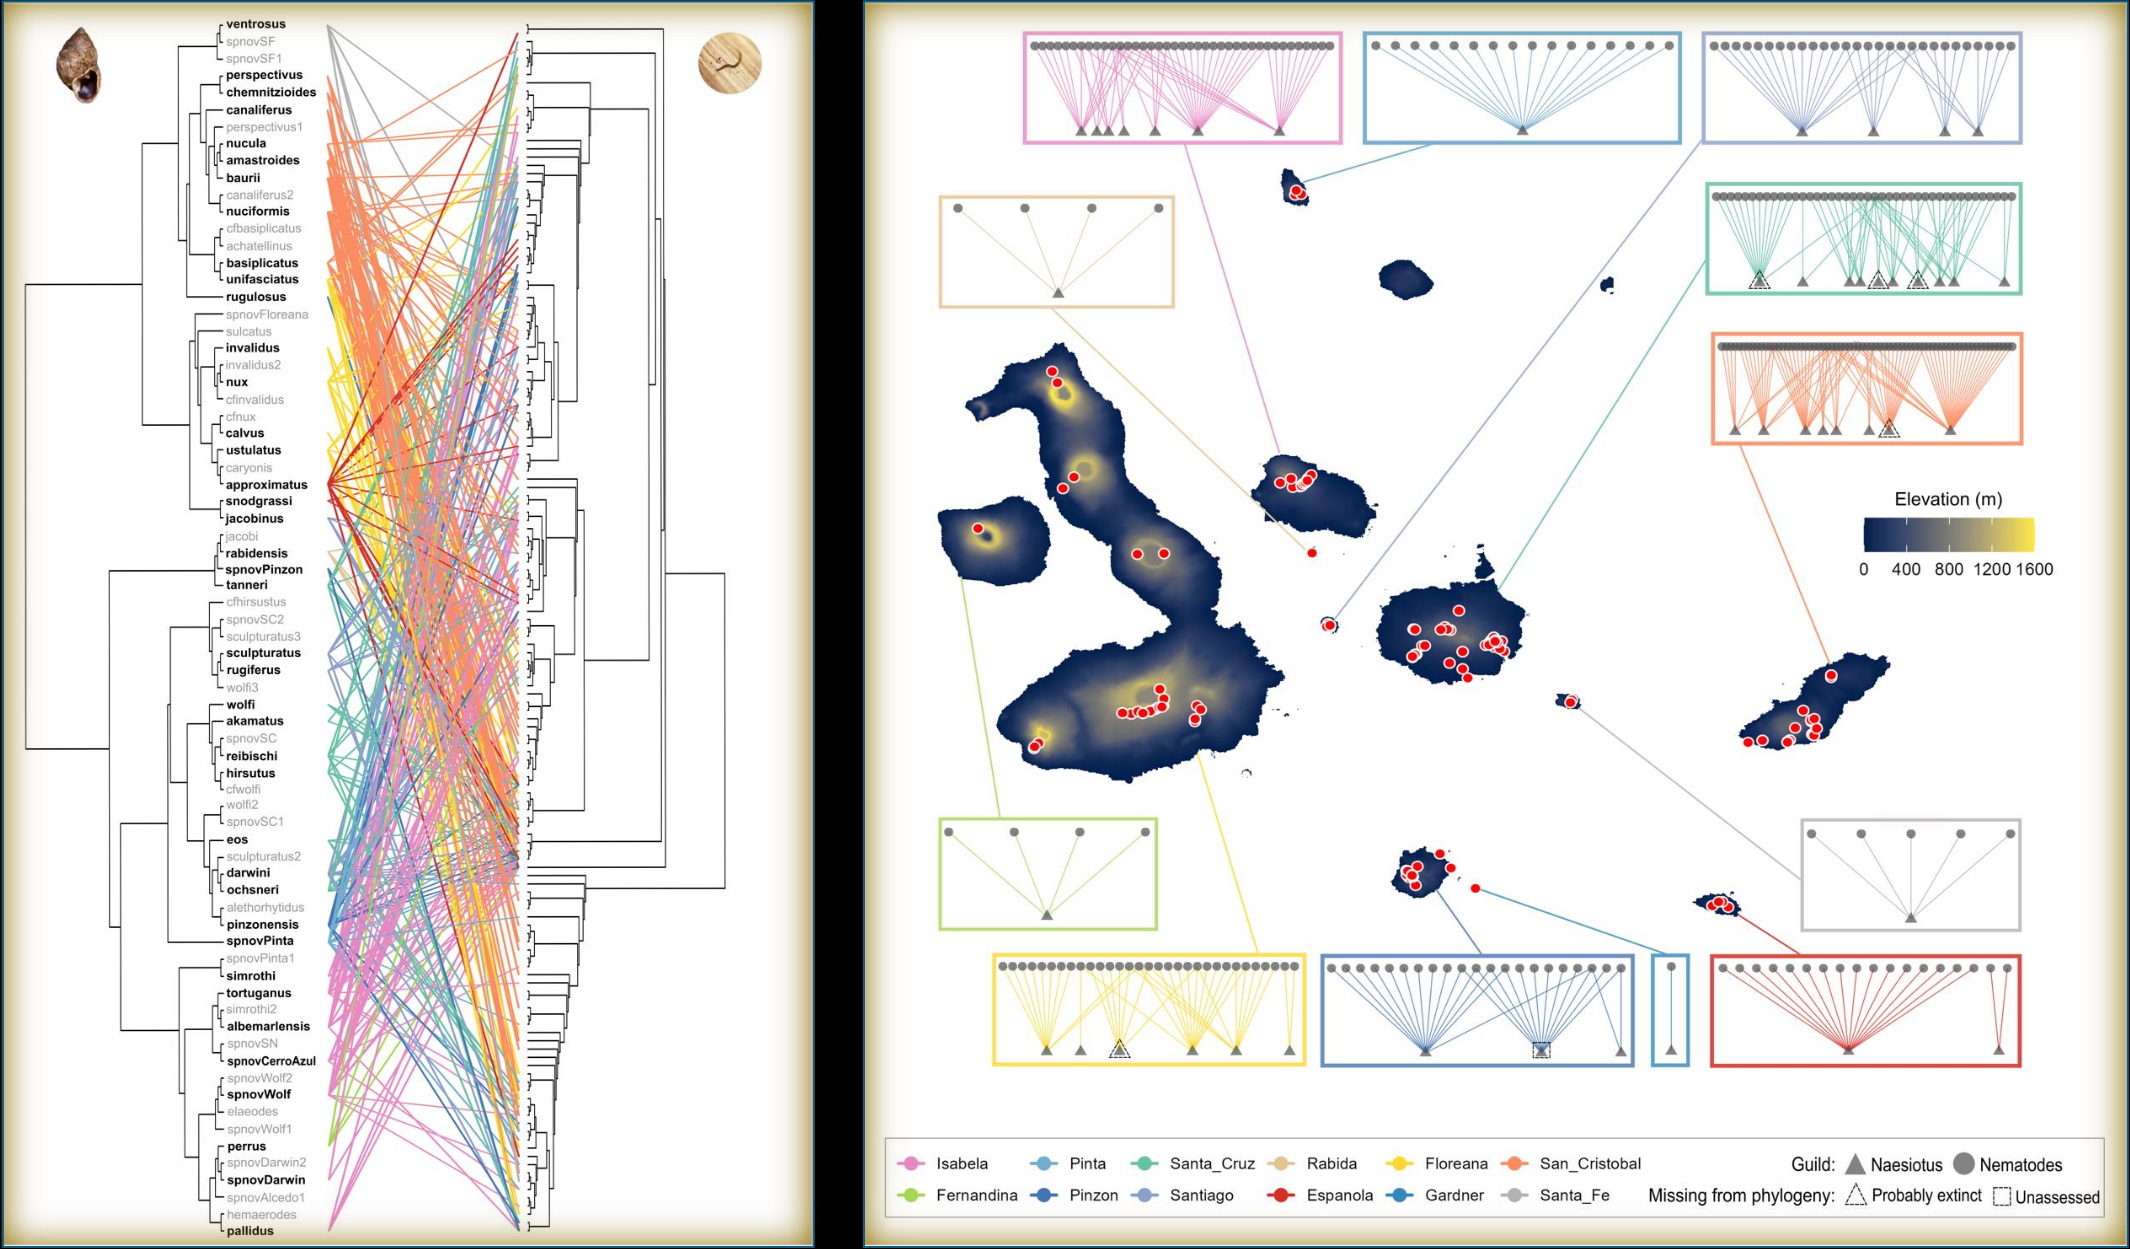
\includegraphics[height=0.7\textheight]{Figs/fuster2026}\\	
		\footnotesize{Fuster et al. 2026. Am. Nat.}
	\end{center}  

\end{frame}

%------------------------------

\begin{frame}{Phylogenetic signal in Galapagos food webs}
	\begin{columns}
		\begin{column}{0.6\textwidth}	
			\begin{center}
				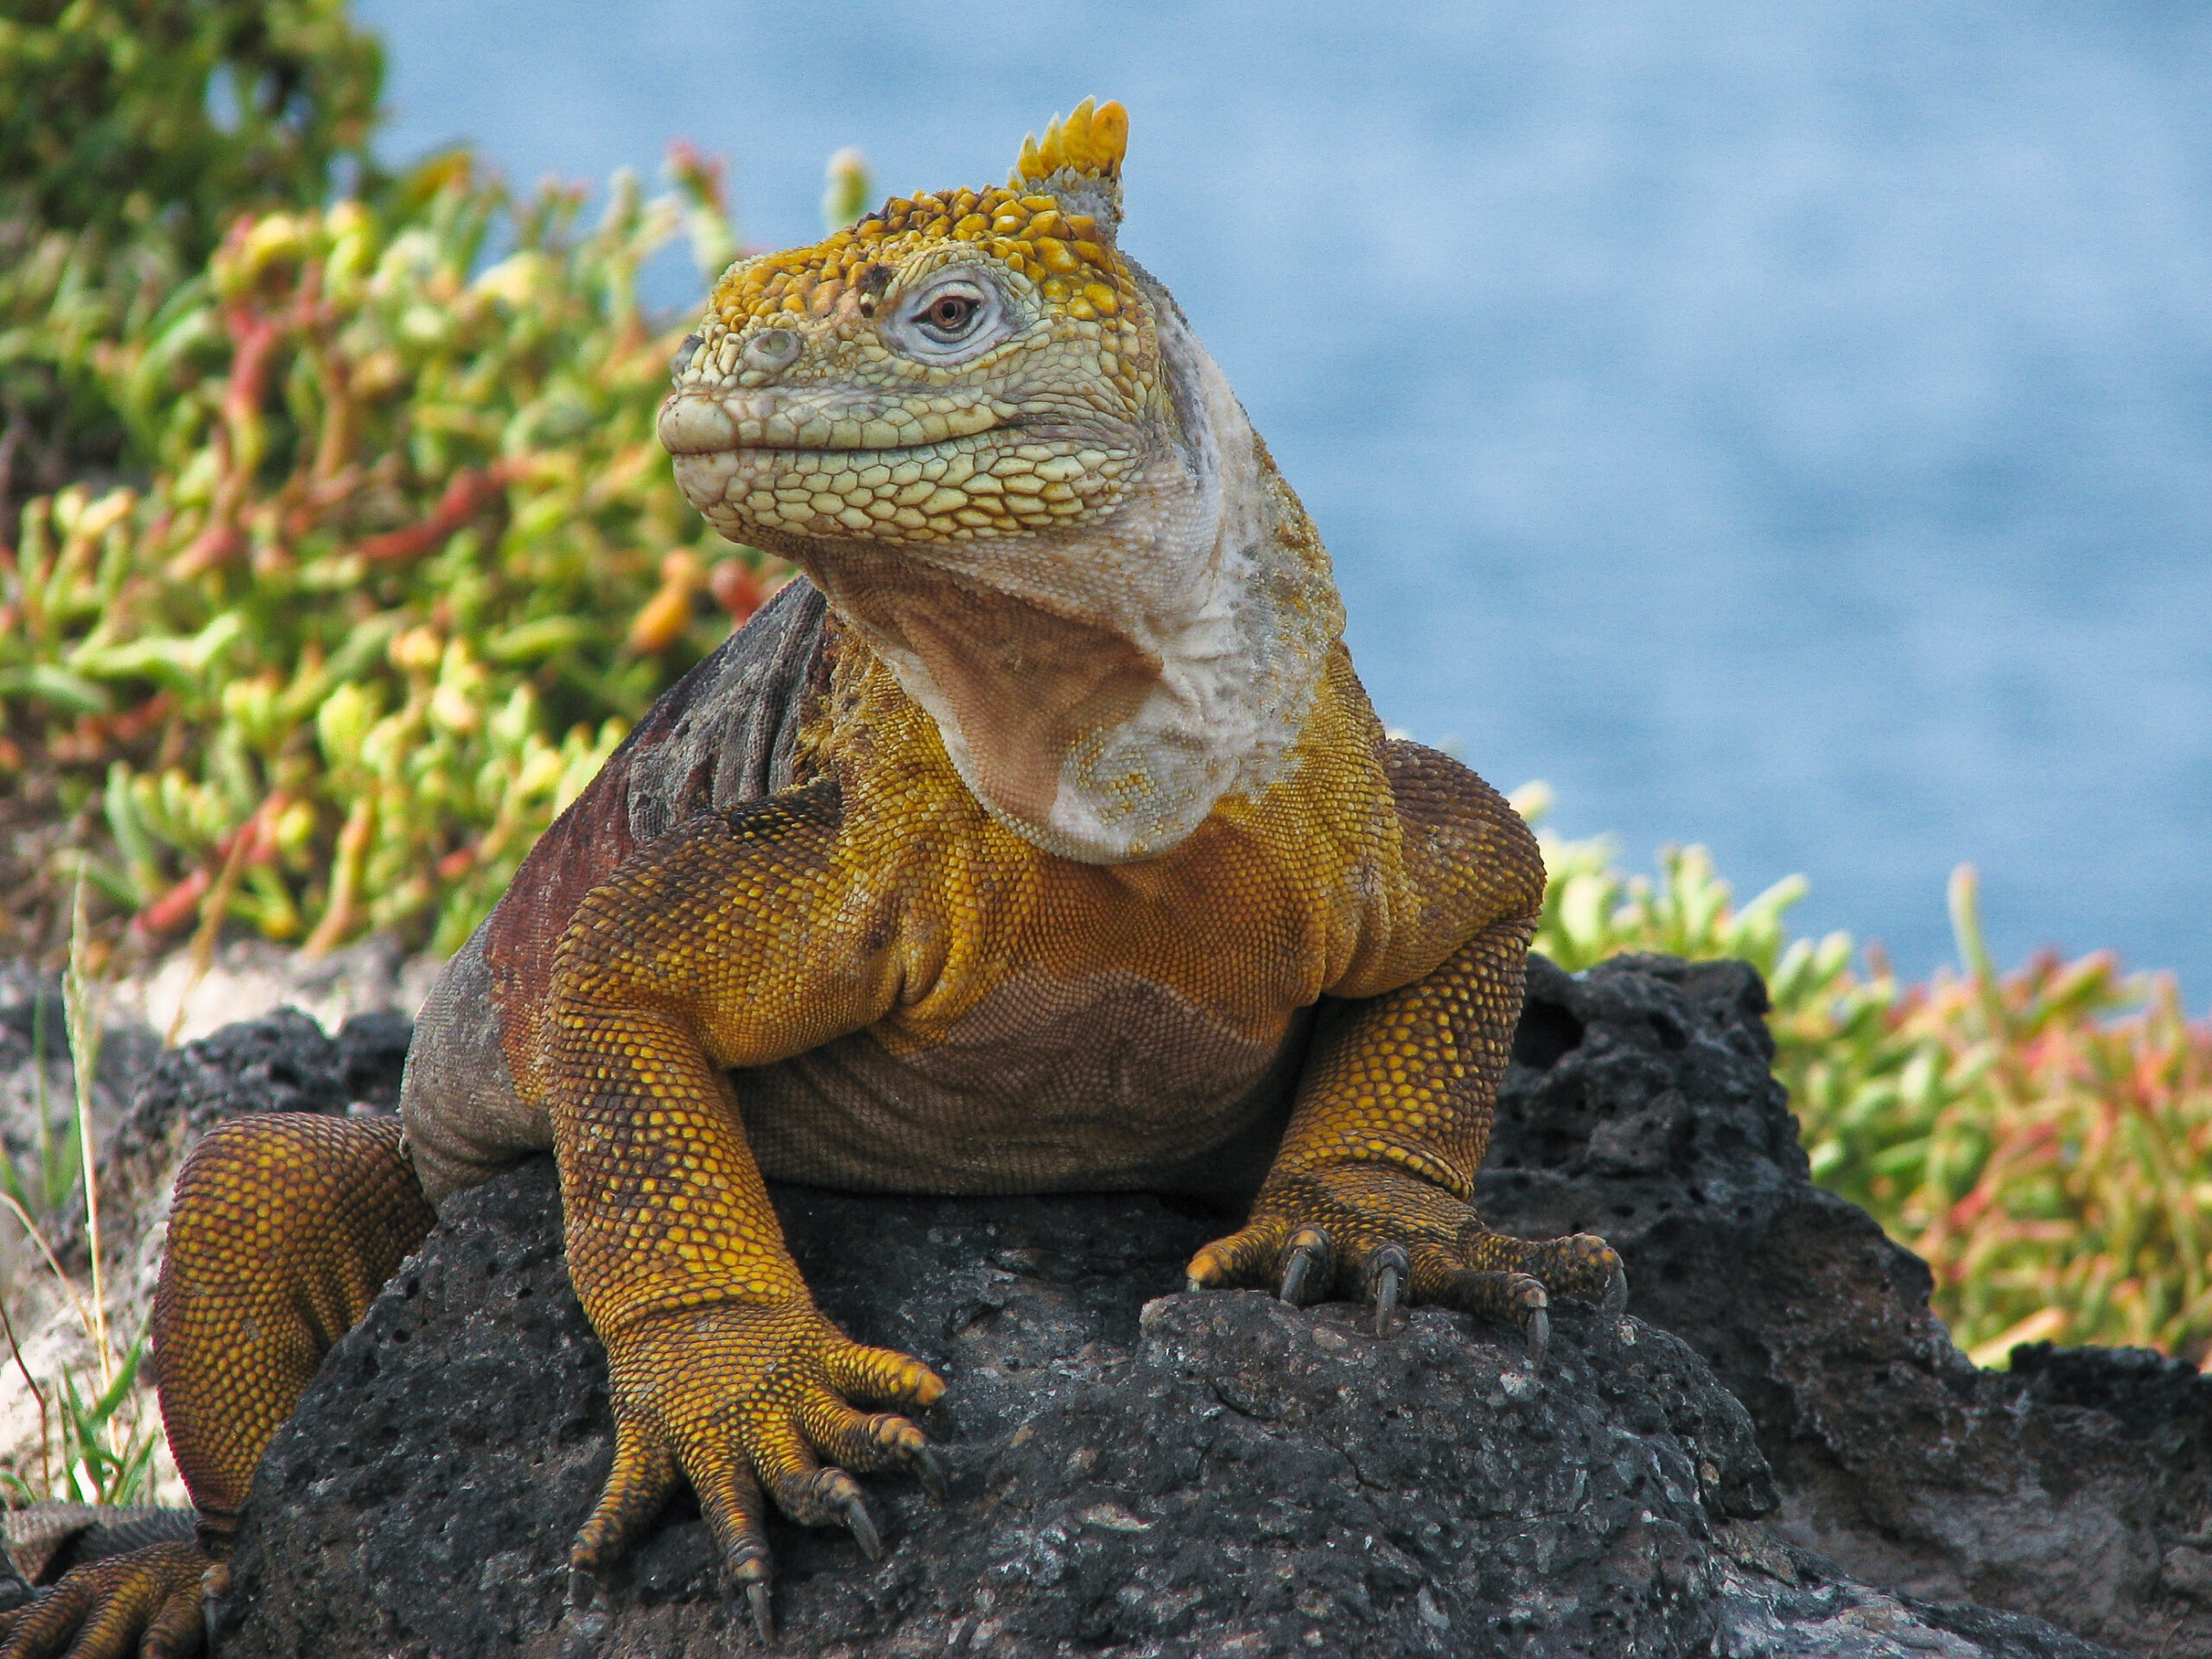
\includegraphics[height=0.55\textheight]{Figs/iguana}\\	
			\end{center}  
		\end{column}
%----
		\begin{column}{0.4\textwidth}						
			\begin{center}
				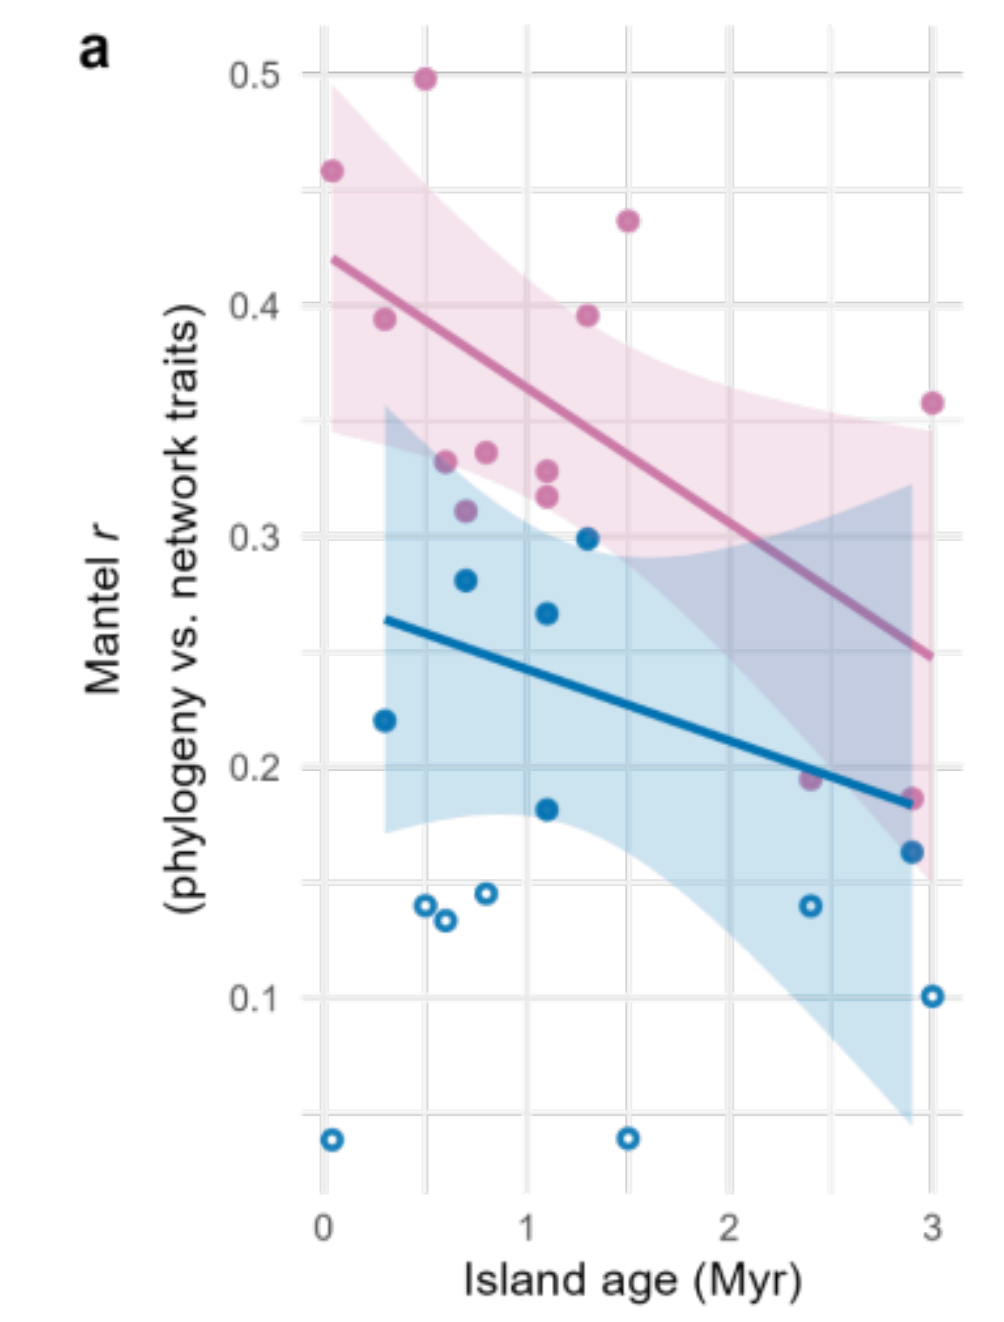
\includegraphics[height=0.7\textheight]{Figs/fuster2025b}\\	
                \footnotesize{Fuster et al. 2026. Am. Nat.}
			\end{center}  
		\end{column}				
	\end{columns} 	
\end{frame}


%------------------------------
% CONCLUSION
%------------------------------

{
\usebackgroundtemplate{}
\begin{frame}

	\pagecolor{BDQC1st}
	\color{white}

	\LARGE{\textit{Conclusion}}

\end{frame}
}

%------------------------------

\begin{frame}{Conclusion}
	\begin{itemize}
		\item Island biogeography theory can be expanded without sacrifying simplicity
		\item The key is to represent trait-dependence of colonization and extinction processes
		\item Local trait distributions are non-random samples of the regional pool
		\item Wide range of predictions, from species-area relationships to phylogenetic structure
	\end{itemize}
\end{frame}

%------------------------------------------------------------------------------------------

\begin{frame}{Looking forward}{From functional anomalies to ecosystem functions}
	\begin{center}
		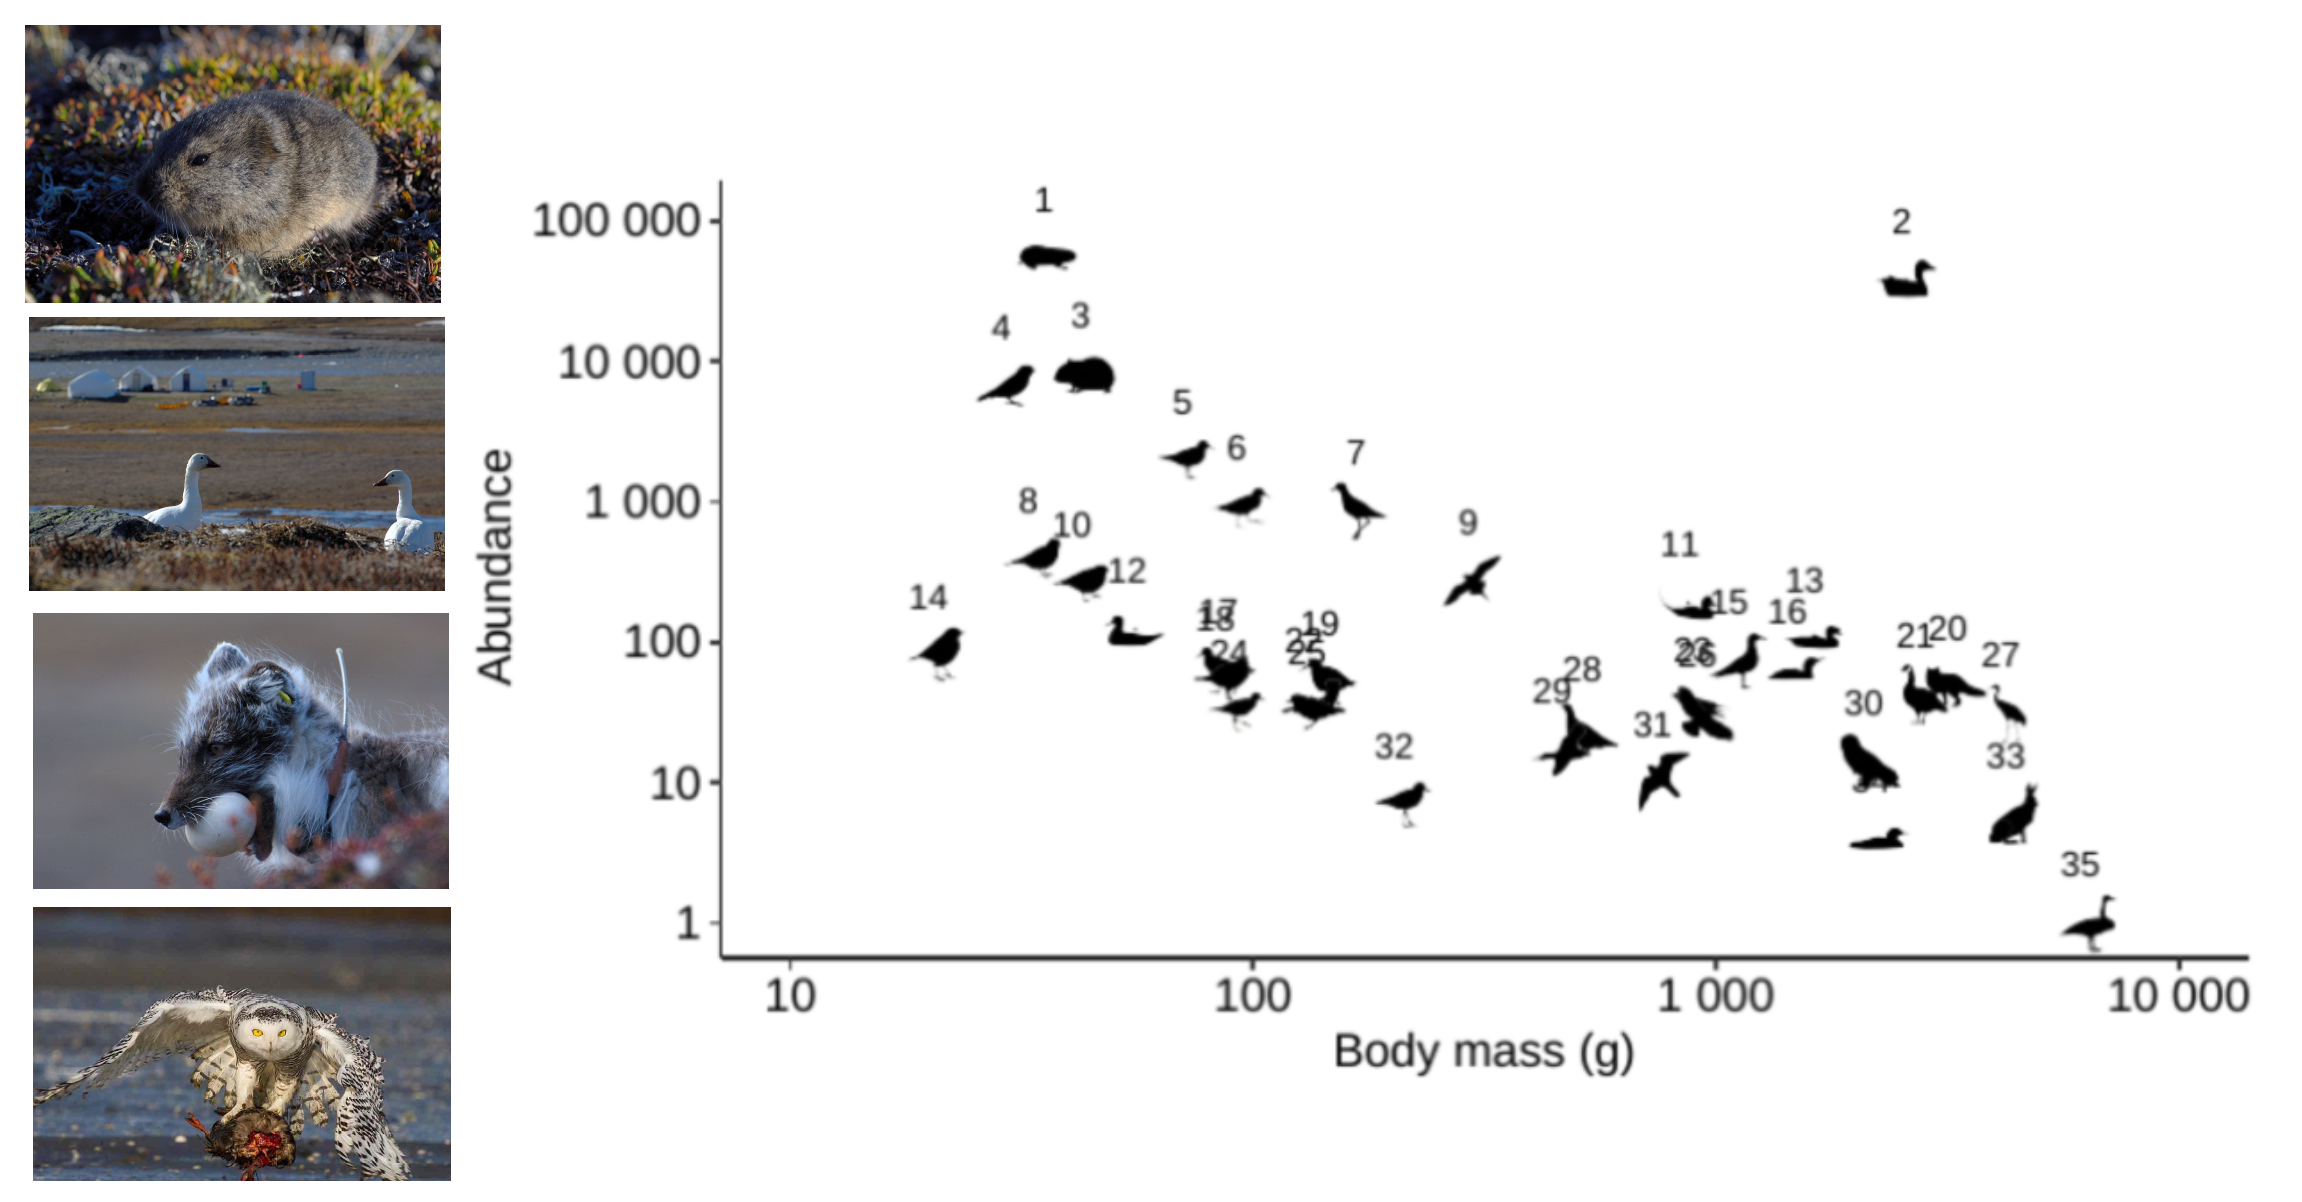
\includegraphics[height=0.65\textheight]{Figs/bylot}\\
	\end{center}  
\end{frame}

%------------------------------
%------------------------------
%------------------------------
\end{document}
